%
% Szakdolgozatminta az Eszterházy Károly Katolikus Egyetem
% matematika illetve informatika szakos hallgatóinak.
%

\documentclass[
% opciók nélkül: egyoldalas nyomtatás, elektronikus verzió
% twoside,     % kétoldalas nyomtatás
% tocnopagenum,% oldalszámozás a tartalomjegyzék után kezdődik
]{thesis-ekf}
\usepackage[T1]{fontenc}
\PassOptionsToPackage{defaults=hu-min}{magyar.ldf}
\usepackage[magyar]{babel}
\usepackage{mathtools,amssymb,amsthm,pdfpages}
\footnotestyle{rule=fourth}

\newtheorem{tetel}{Tétel}[chapter]
\theoremstyle{definition}
\newtheorem{definicio}[tetel]{Definíció}
\theoremstyle{remark}
\newtheorem{megjegyzes}[tetel]{Megjegyzés}

\begin{document}

\institute{Matematikai és Informatikai Intézet}
\title{KRESZ alapú tanulás segítő játék fejlesztése Unity keretrendszerben}
\author{Fodor Győző Benedek\\Programtervező Informatikus Bsc.}
\supervisor{Troll Ede Mátyás\\Tanársegéd}% beosztások: mestertanár, tanársegéd, adjunktus, főiskolai docens, egyetemi docens, főiskolai tanár, egyetemi tanár
\city{Eger}
\date{2026}
\maketitle

\tableofcontents

\chapter*{Bevezetés}
\addcontentsline{toc}{chapter}{Bevezetés}
A szakdolgozatom témáját akkor kellett választanom, amikor a szabadidőm nagy részét a jogosítványom megszerzésére fordítottam. A szabályok megértése és megtanulása egyszerű volt, de az úton, a közlekedési helyzetekben való alkalmazásuk már sokkal bonyolultabb. Az úgynevezett ,,3 pontos'' feladatok, amik egy KRESZ vizsga jelentős részét alkotják, erre alapulnak. Az ilyen feladványok játékos gyakorlására akartam megoldást találni. 

Egy olyan felületet szerettem volna létrehozni ami magába tudja foglalni egy közlekezdési szituáció minden elemét. Fontos hogy a részletek könnyen felismerhetőek legyenek, és az egész jelenet interaktív legyen, segítve az adott helyzetben érvényesülő szabályok megértését. A tervem megvalósítására a Unity keretrendszert találtam a legalkalmasabbnak.

\begin{figure}[ht!]
	\centering
	\begin{minipage}{7.5cm}
		\centering
		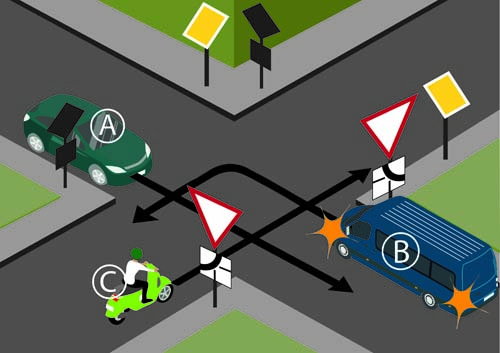
\includegraphics[height=5cm]{images/harompontos}
		\caption{Három pontos feladat (szuperjogsi.hu) \cite{harompontos}}
	\end{minipage}
\end{figure}
A szakdolgozat kódja, a hozzá tartozó build, és a játék működését bemutató videó a itt található:

Forráskód: https://github.com/FourthRuffle/KRESZTraffic-thesis

Build: https://github.com/FourthRuffle/KRESZTraffic-thesis

Videó: https://youtu.be/Q9aeaCG2Be4

\chapter{Technológiai áttekintés}
A 20.~század alkonyán a játékfejlesztők még sokkal kevesebben és kisebb erőforrásból dolgoztak, így sokkal gyakoribb volt, hogy a játékaikhoz saját motort fejlesztettek, mivel akkoriban nem sok kész, piaci játékmotor volt elérhető. Nagy segítség lehetett viszont, ha valaki meg tudott vásárolni egy kész kódbázist.

Ilyen volt például az \textit{id Software} cég fejlesztette ,,id Tech'' motor, melynek később több verciója is készült. Ezeket a motorokat használták az első meghatározó FPS~(first~person shooter) játékok mint például \textit{DOOM}, \textit{Quake}, \textit{Wolfenstein} sorozatok alapjául.\cite{id_software}

\begin{figure}[ht!]
	\centering
	\begin{minipage}{7.5cm}
		\centering
		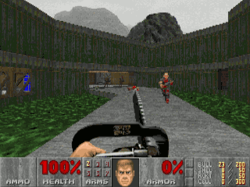
\includegraphics[height=5cm]{images/doom}
		\caption{Korai képernyőkép a DOOM játékból (DOOM 1993) \cite{doom}}
	\end{minipage}
\end{figure}
\newpage
\section{Unreal Engine}

Az \textit{Unreal Engine} az mai napig egyik legmeghatározóbb játékmotor. Az Epic Games játékfejlesztő cég 1998-ban készítette az \textit{Unreal} nevú játékukhoz. Azóta 4-5 évente jelent meg új verzió, ami mindig jelentős változásokat hozott a aktuális játékiparba. 

\begin{figure}[ht!]
		\centering
		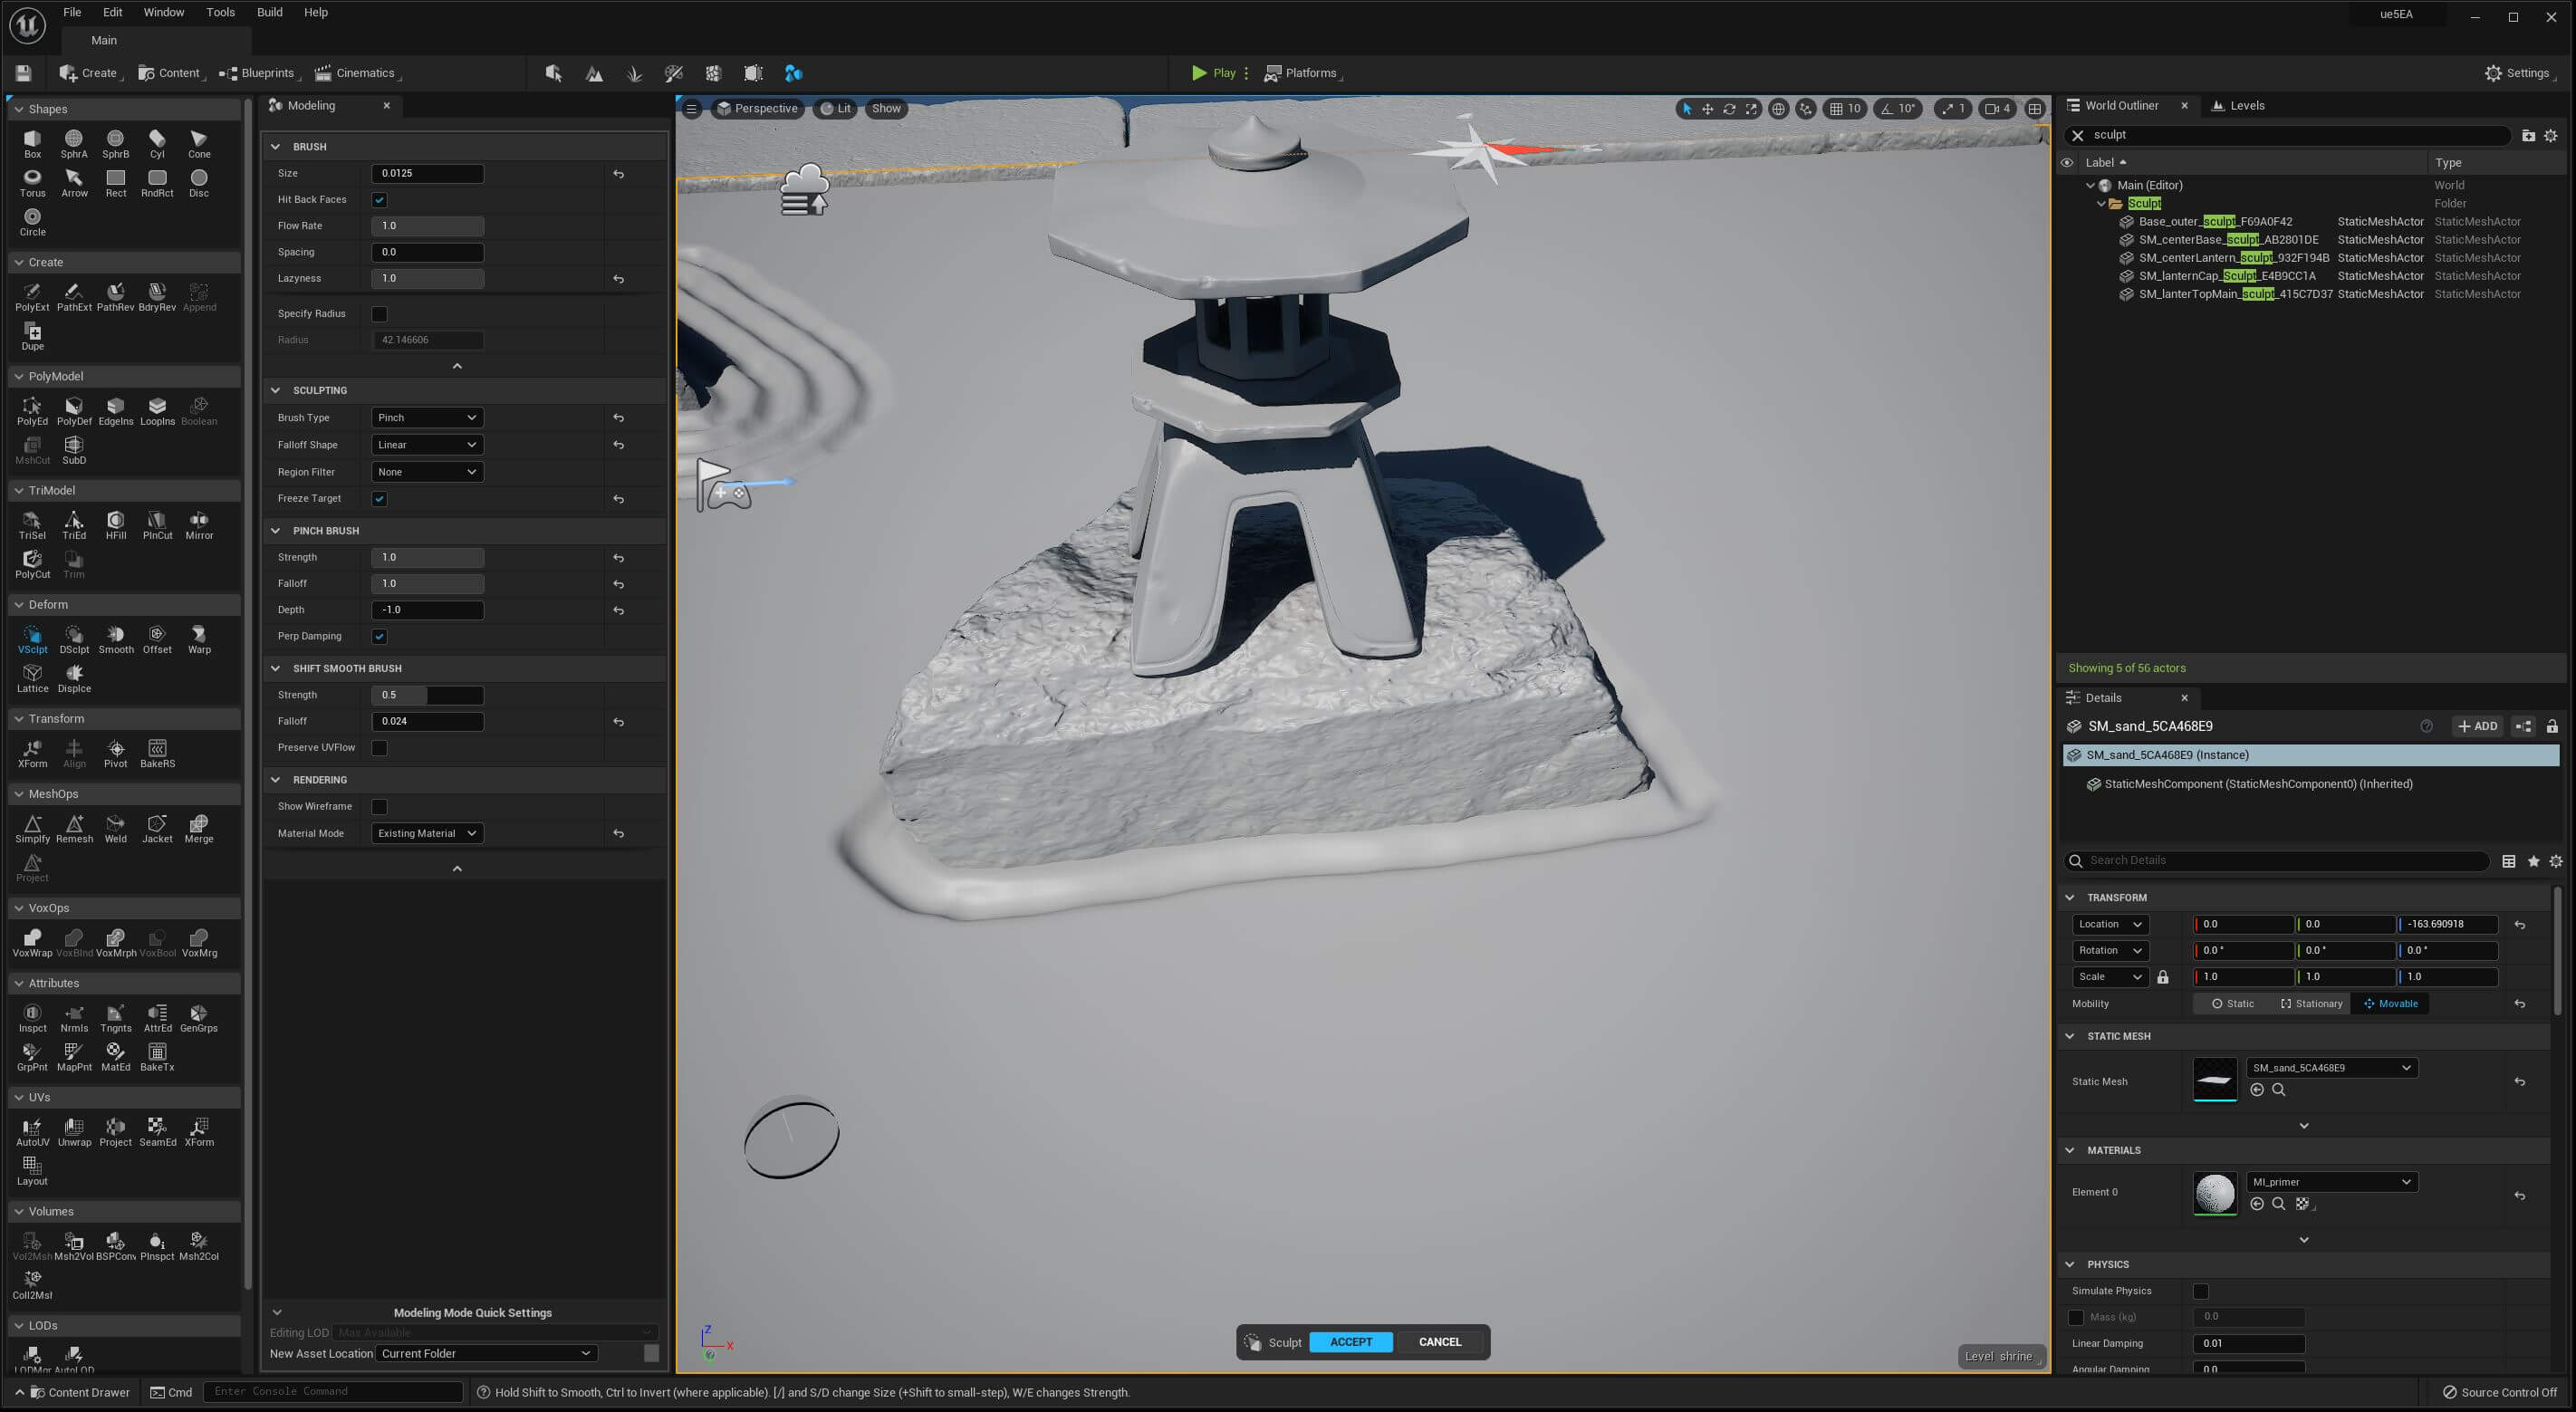
\includegraphics[height=5cm]{images/unreal}
		\caption{Unreal Engine kezőfelület (unrealengine.com) \cite{unreal_img}}
\end{figure}

Eredetileg az \textit{Unreal Engine} is az FPS genre kiszolgálására készült. Később viszont a TPP (third person perspective) féle kalandjátékok és rengeteg más 3D-s játék alapjául is szolgált, legyen az lövöldözős, kaland, nyílt világ, vagy történet műfajú.

A motor a mai napig C++ nyelven működik, 2012-ig Java-val társítva az \textit{UnrealScript}-et használta, azonban ezt lecserélték és azóta a \textit{Blueprint} vizuális programozási felület a fejlesztők barkácsolóasztala. 

Az alapvetően ingyenes szoftver legújabb, 2022-es verziójának  forráskódja a GitHub-on is elérhető, viszont a kereskedelmi felhasználás jogdíj köteles, amit az Epic Games a bevétel 5\%-aként határozott meg. \cite{unity_engine}
\section{Godot}
Egy másik szintén ingyenesen hozzáférhető és népszerű játékmotor a \textit{Godot}. \textit{Juan Linietsky} fejlesztette és adta ki először 2001-ben. A motor több néven is ismerté vált, majd 2014-ben felkerült GitHubra. Napjainkban a fejlesztés a 4.0-ás verziónál tart, ahol a 3D-s felületet igyekeznek felzárkóztatni a versenytársakhoz. 

\begin{figure}[ht!]
		\centering
		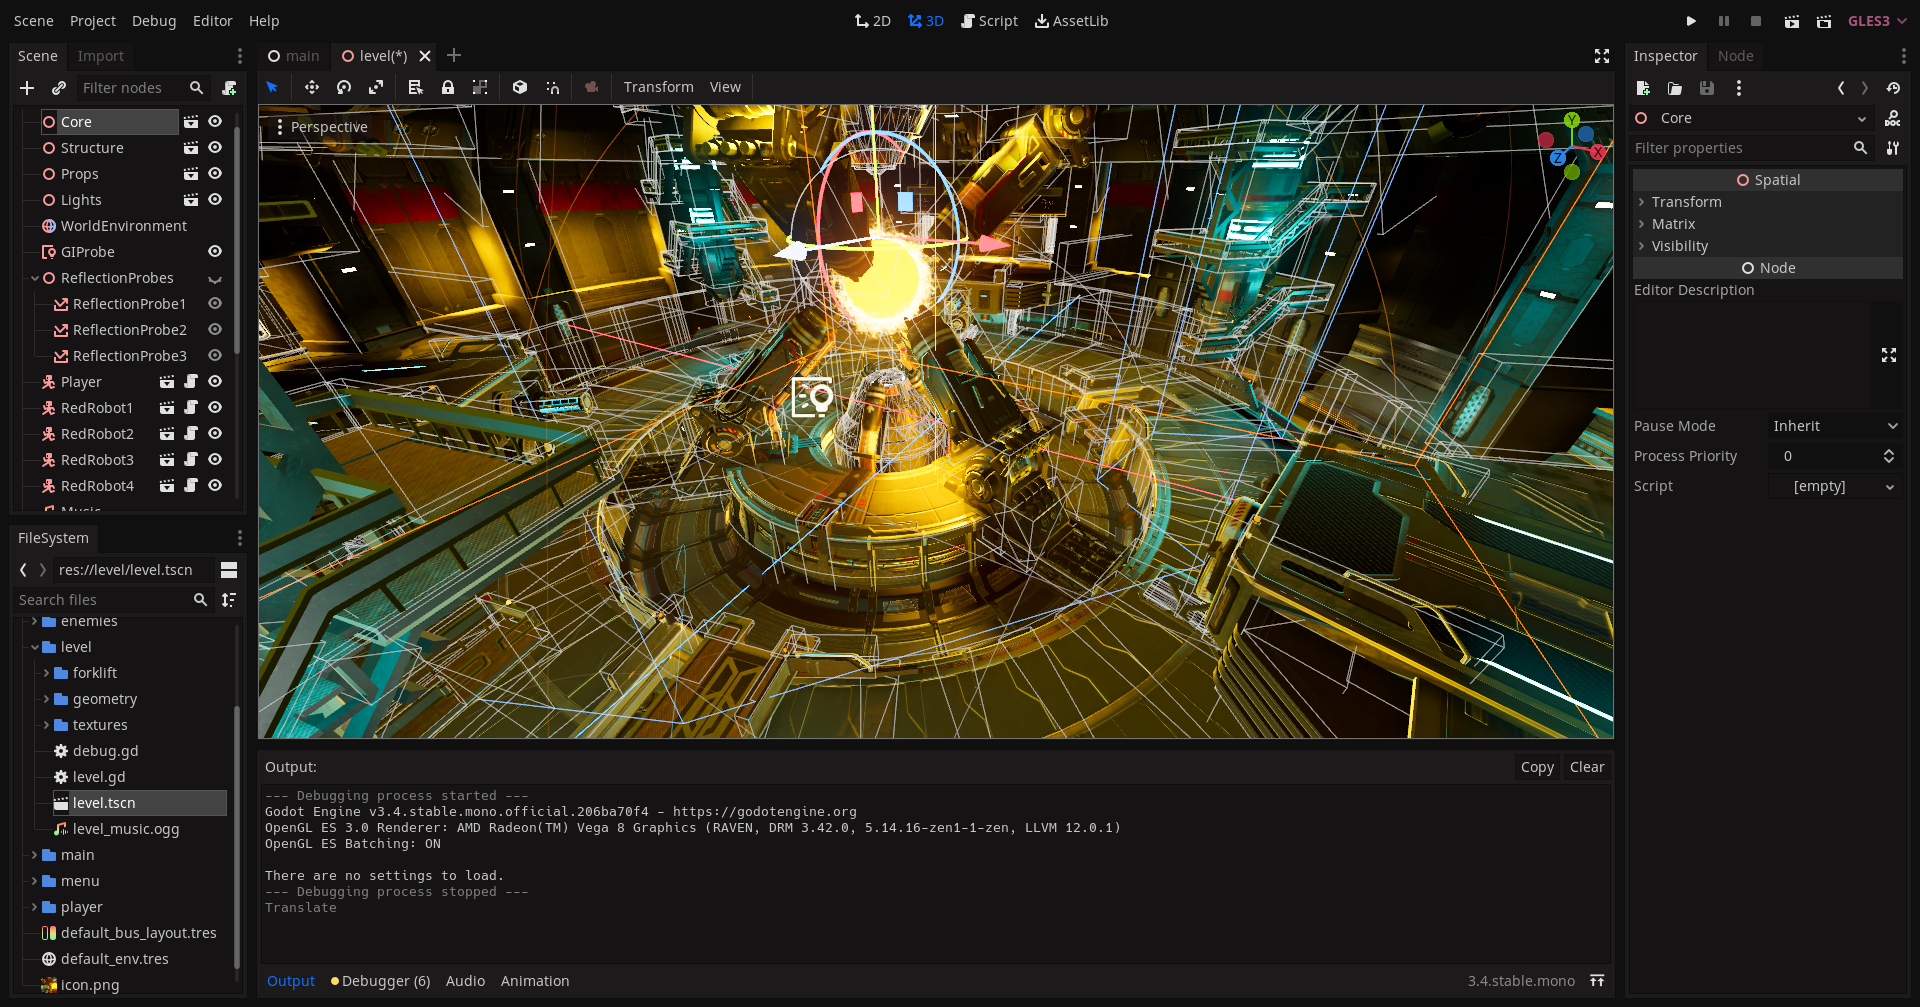
\includegraphics[height=5cm]{images/godot}
		\caption{Godot kezőfelület (Godot 4.6 2026) \cite{godot_img}}
\end{figure}

A motor nem csak egy programozási nyelvhez kötött, de a három leggyakoribb a C++ és C\#, valamit a GDSript. A GDScript a Godot saját rendszeréhez optimalizált objektum orientált programozási nyelv, a Pythonhoz hasonló struktúrával. A vizuális programozás opciója itt is megjelenik, régebben a \textit{VisualScript}-ként, ez viszont a 4.0-ás verzióban már nem elérhető. \cite{godot_engine}
\section{Unity}
A Unity a \textit{Unity Technologies} fejlesztői által készített ingyenesen használható játékmotor. A motor támogatása kiterjed a számítógépeken kívül a konzolokra és okostelefonokra is. A 2D-s és 3D-s alkalmazások készítésére is alkalmas fejlesztői környezet hamar elterjedt a mobilfejlesztők és a feltörekvő, egy vagy több személyes kis fejlesztőcsapatok körében. A Unity felépítése könnyen megérthető és a C\# programozási nyelv is gyorsan tanulható, emellett rengeteg oktatóvideó és kurzus is segíti a kezdőket az alapok elsajátításában.\cite{unity_engine}

\begin{figure}[ht!]
		\centering
		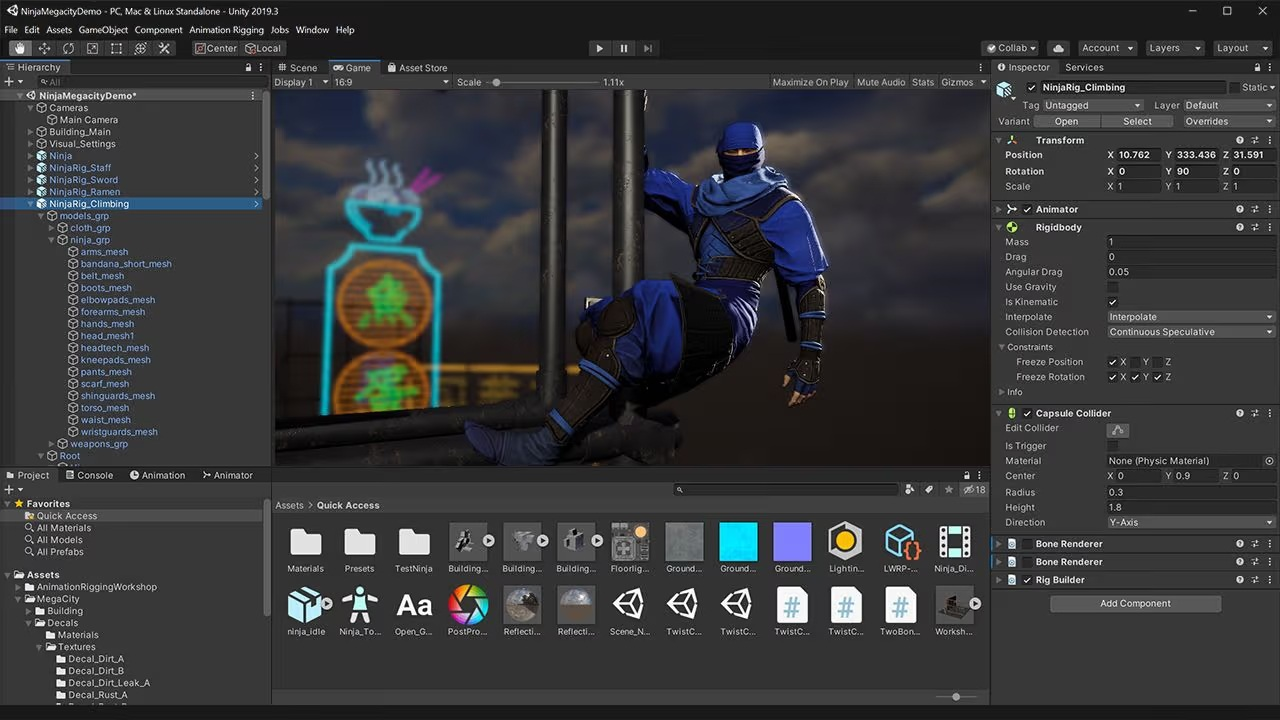
\includegraphics[height=5cm]{images/unity}
		\caption{Unity kezőfelület (2026) \cite{unity_img}}
\end{figure}

A fejlesztőcég először \textit{Over The Edge Entertainment} jelent meg, csak 2007-ben nevezték át \textit{Unity Technologies}-ra. \cite{unity_technologies}

A legjelentősebb fejlesztései:
\begin{itemize}
	\item 2010: \textit{Unity Asset Store}. Egy ,,Piac'', ahol a Unity-ben való fejlesztéshez használható fájlokat találhatsz ingyenesen és díjazva is.
	\item 2018: \textit{Unity Hub}. Egy külön felület, ahol a Unity projekteket kezelheted és a motor különböző verziói közötti navigálást is megkönnyíti.
\end{itemize} 

\begin{figure}[ht!]
		\centering
		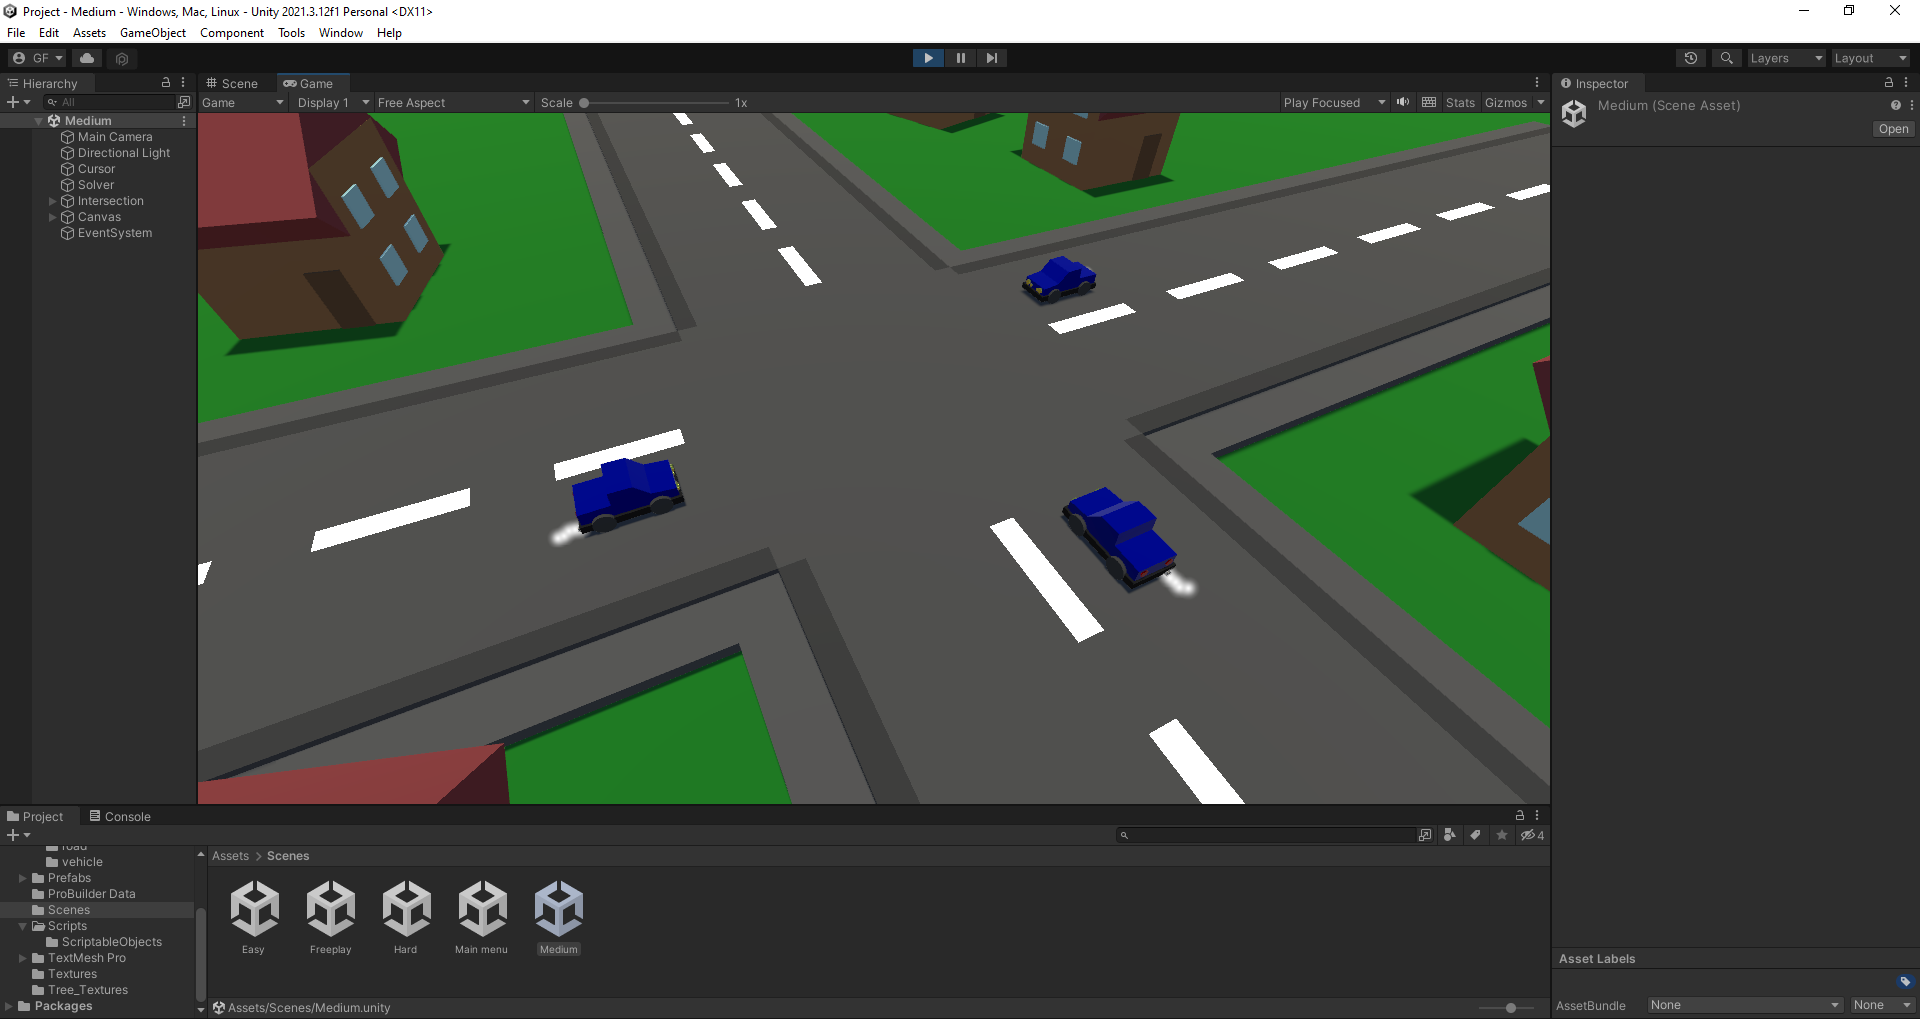
\includegraphics[height=5cm]{images/unity_sajat}
		\caption{Unity kezőfelület (Saját projekt)}
\end{figure}


\subsection{Komponensek}
A Komponensek a Unity egyik fő résztvevői. A komponens tulajdonságai teszik lehetővé, hogy egy \textit{GameObject} személyre szabható legyen. A GameObject-ek építik fel a játékokat, ezek a fő elemei a kész programnak. Sok komponens mint például a \textit{Transform} vagy a \textit{Collider}-ek, kevesebb funkciót ágyaznak magukba vagy rengetegszer felbukkanhatnak a program során. \cite{unity_components}

A Unity a saját komponensek létrehozását is lehetővé teszi, ezáltal kivételes szabadságot adva a fejlesztőnek. Amennyiben ezeknek a komponenseknek őse a \textit{MonoBehaviour} osztály, az összes többi GameObject-re rácsatolhatóvá válnak és így új funkciókat adhatunk az adott objektumnak. \cite{unity_monobehaviour}
\newpage
\section{Közlekedési szabályok}
A Közúti Rendelkezések Egységes Szabályozása (rövidítve: KRESZ) az a  közlekedési szabálygyűjtemény amely a Magyarország területén levő közutakon és közforgalom elől el nem zárt magánutakon folyó közlekedést szabályozza.

A közúti forgalom rendjét már a 19. században elkezdték meghatározni. Az első magyar KRESZ egy 1910-ben született belügyminiszteri rendelet ami az azt egy évvel megelőző \textit{Párizsi egyezmény} alapjaira készült. Ekkor még csak töredéke volt a mai szabályrendszernek. Ami viszont már ebben a korban és megjelent a KRESZ-ben az az autók műszaki vizsgálata és rendszámozása, a gépjárművezetők képzése, valamint az első négy közúti jelzőtábla:
\begin{itemize}
	\item útkereszteződés
	\item kanyar
	\item vasúti átjáró
	\item bukkanó
\end{itemize}
1941-ben vezették be a jobboldali közúti közlekedést és ezzel együtt az úgynevezett ,,Jobbkéz szabályt''. 

\begin{figure}[ht!]
		\centering
		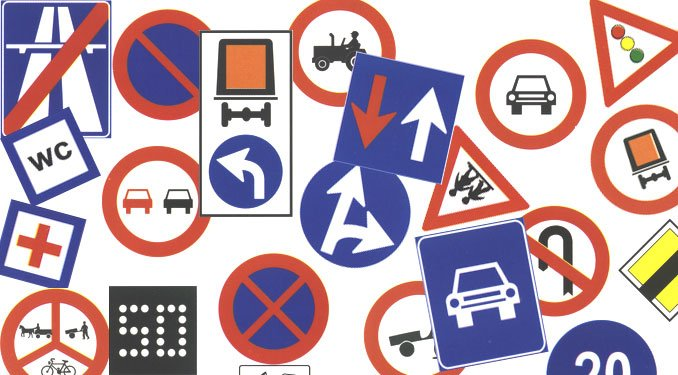
\includegraphics[height=5cm]{images/kresz}
		\caption{KRESZ táblák \cite{kresz_img}}
\end{figure}

\chapter{Rendszerterv}

\section{A rendszer célja}
A szakdolgozat célja egy olyan játék létrehozása, amiben a KRESZ vizsgák és tananyagokban szereplő ,,3-pontos'' feladatokat játékos módon érthetőbbé, átláthatóbbá és tanulhatóbbá teszi. Fontos, hogy a játékos tudja tesztelni a tudását, a játék pedig interaktív és reszponzív legyen.

\section{Telepítés}
A nem szükséges telepíteni a játékszoftvert, egyből a kicsomagolás után indítható a mappában található alkalmazással.
\section{Fejlesztéshez használt eszközök}
\begin{itemize}
	\item Unity: A játék készítéséhet használt fejlesztői környezet. Verzió: 2021.3.12f1
	\item Visual Studio: A programozói környezet, amely Unity támogatással rendelkezik. Verzió: Community 2022
	\item Visual Studio, WinForms: Vizuális fejlesztőkörnyezet a Visual Studio-n belül. A program kezdeti algoritmusainak a C\# nyelvben való megvalósításra szolgált.
\end{itemize}
\section{Funkcionális elvárások}
\begin{itemize}
	\item KRESZ alapú szabályrendszer: Egy olyan háttér algoritmus ami a szituációban szereplő objektumokat kezelni. Az algoritmus áthaladási sorrendet állít fel ami egyben a feladvány helyes megoldását is meghatározza. 
	\item Interaktív játékostér: A feladatot alkotó szereplők kattinthatóak legyenek és rendelkezzenek animált mozgással. A játék értesítse a felhasználót a hibás lépésről, vagy helyes megoldásról.	
	\item Szabad játék: Végtelen ismétlődő randomizált feladványok ahol a játékos gyakorolhatja a közlekedési szituációkat.
	\item Nehézségi szintek: Különböző nehézségű feladványok a könnyebben követhető tanulási és gyakorlási görbéhez valamint a monotonitás elkerüléséhez.
	\item Teszt felület: Egy véges ,,Teszt'' mód ahol a gyakorolt feladatokat adott megadott összesített sikerességi rátával kell megoldani a teszt teljesítéséhez. Támpont a tudás és gyakorlat fejlődésében. 
	\item Pontrendszer: Mind a szabad játéknak, mind a teszt felületnek megfelelő pontrendszer ami a játékos eredményét rögzíti folyamatosan.
\end{itemize}

\chapter{Játékmenet}
Az indítás után az első megálló a főmenü. Itt választhatjuk ki, hogy a ,,Play'' gombra nyomva egy szabad játékba kezdünk, vagy a ,,Teszt''-el egy tesztet indítunk, ahol megmérettethetjük saját tudásunkat a gyakoroltak alapján.

\begin{figure}[ht!]
	\centering
	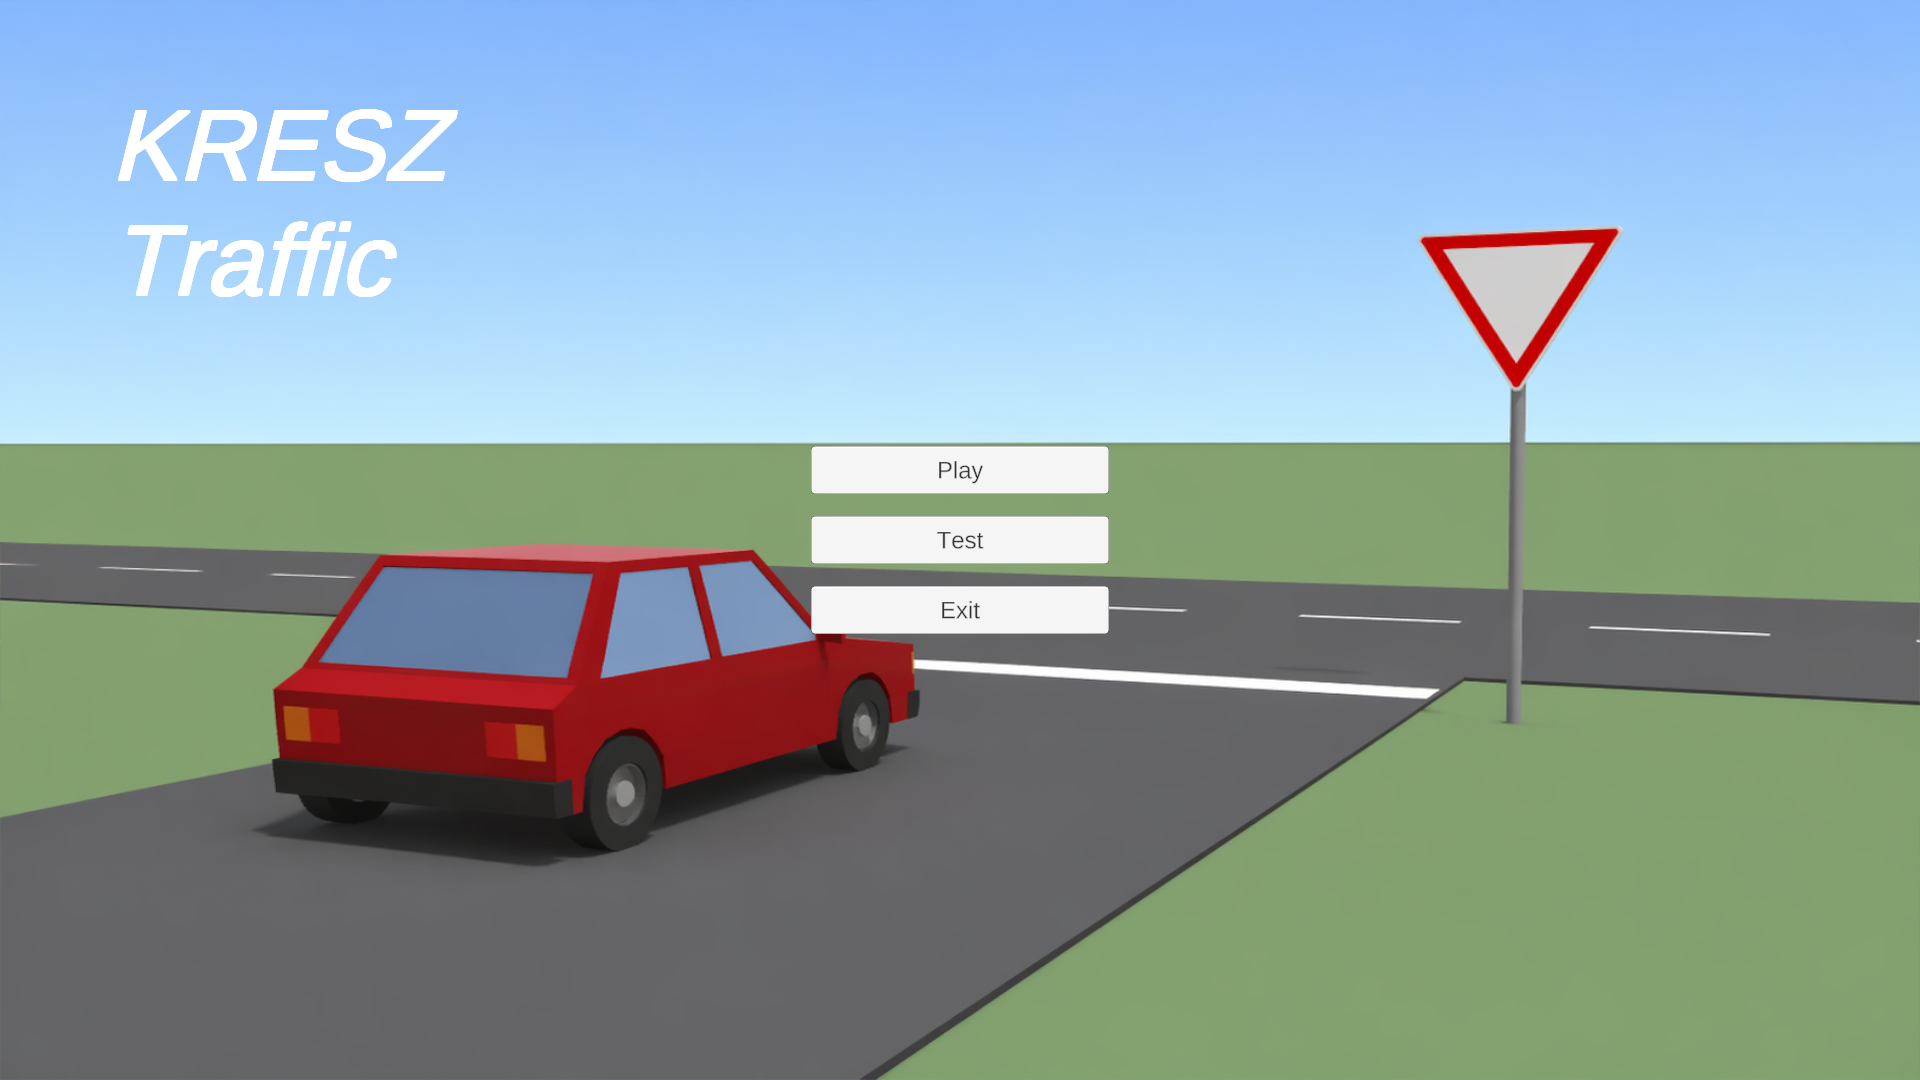
\includegraphics[height=5cm]{images/fomenu}
	\caption{A játék Főmenüje}
\end{figure}

\section{Szabad játék}
A szabad játék egy végtelen játékmód. Itt az összes elérhető variációból véletlenszerűen kiválasztott feladatokat kapunk amiket a közlekedési szituációban résztvevő autókra kattintva kell megoldanunk. Ha helyes sorrendben választjuk ki az autókat, a feladatot teljesítettük, és léphetünk tovább a következőre.

\begin{figure}[ht!]
	\centering
	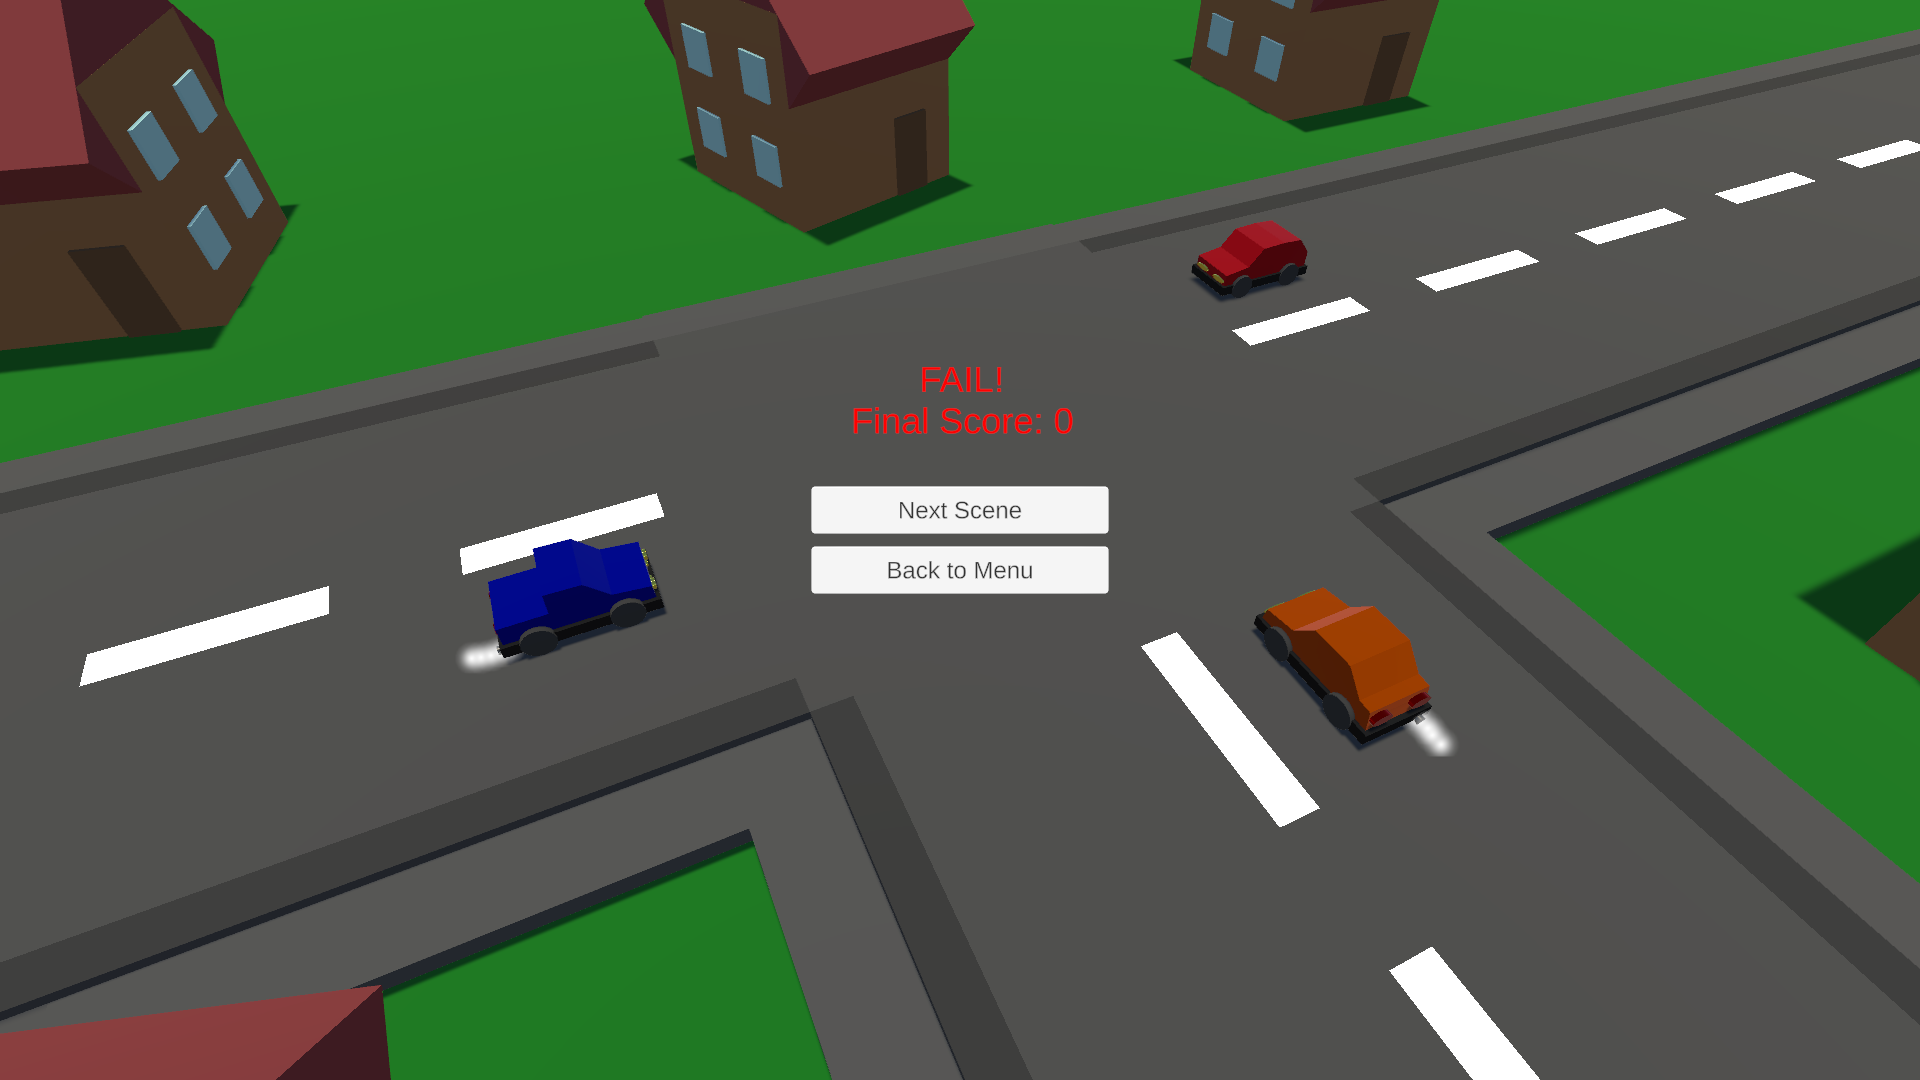
\includegraphics[height=5cm]{images/fail}
	\caption{Hibásan megoldott feladat a szabad játékban}
\end{figure}

Minden sikeresen megoldott feladat után egy pont jár, az ide tartozó pontrendszer a játékos aktuális játéka alatt helyesen megoldott feladványait tartja számon egész addig még a játékot be nem fejezik.

\begin{figure}[ht!]
	\centering
	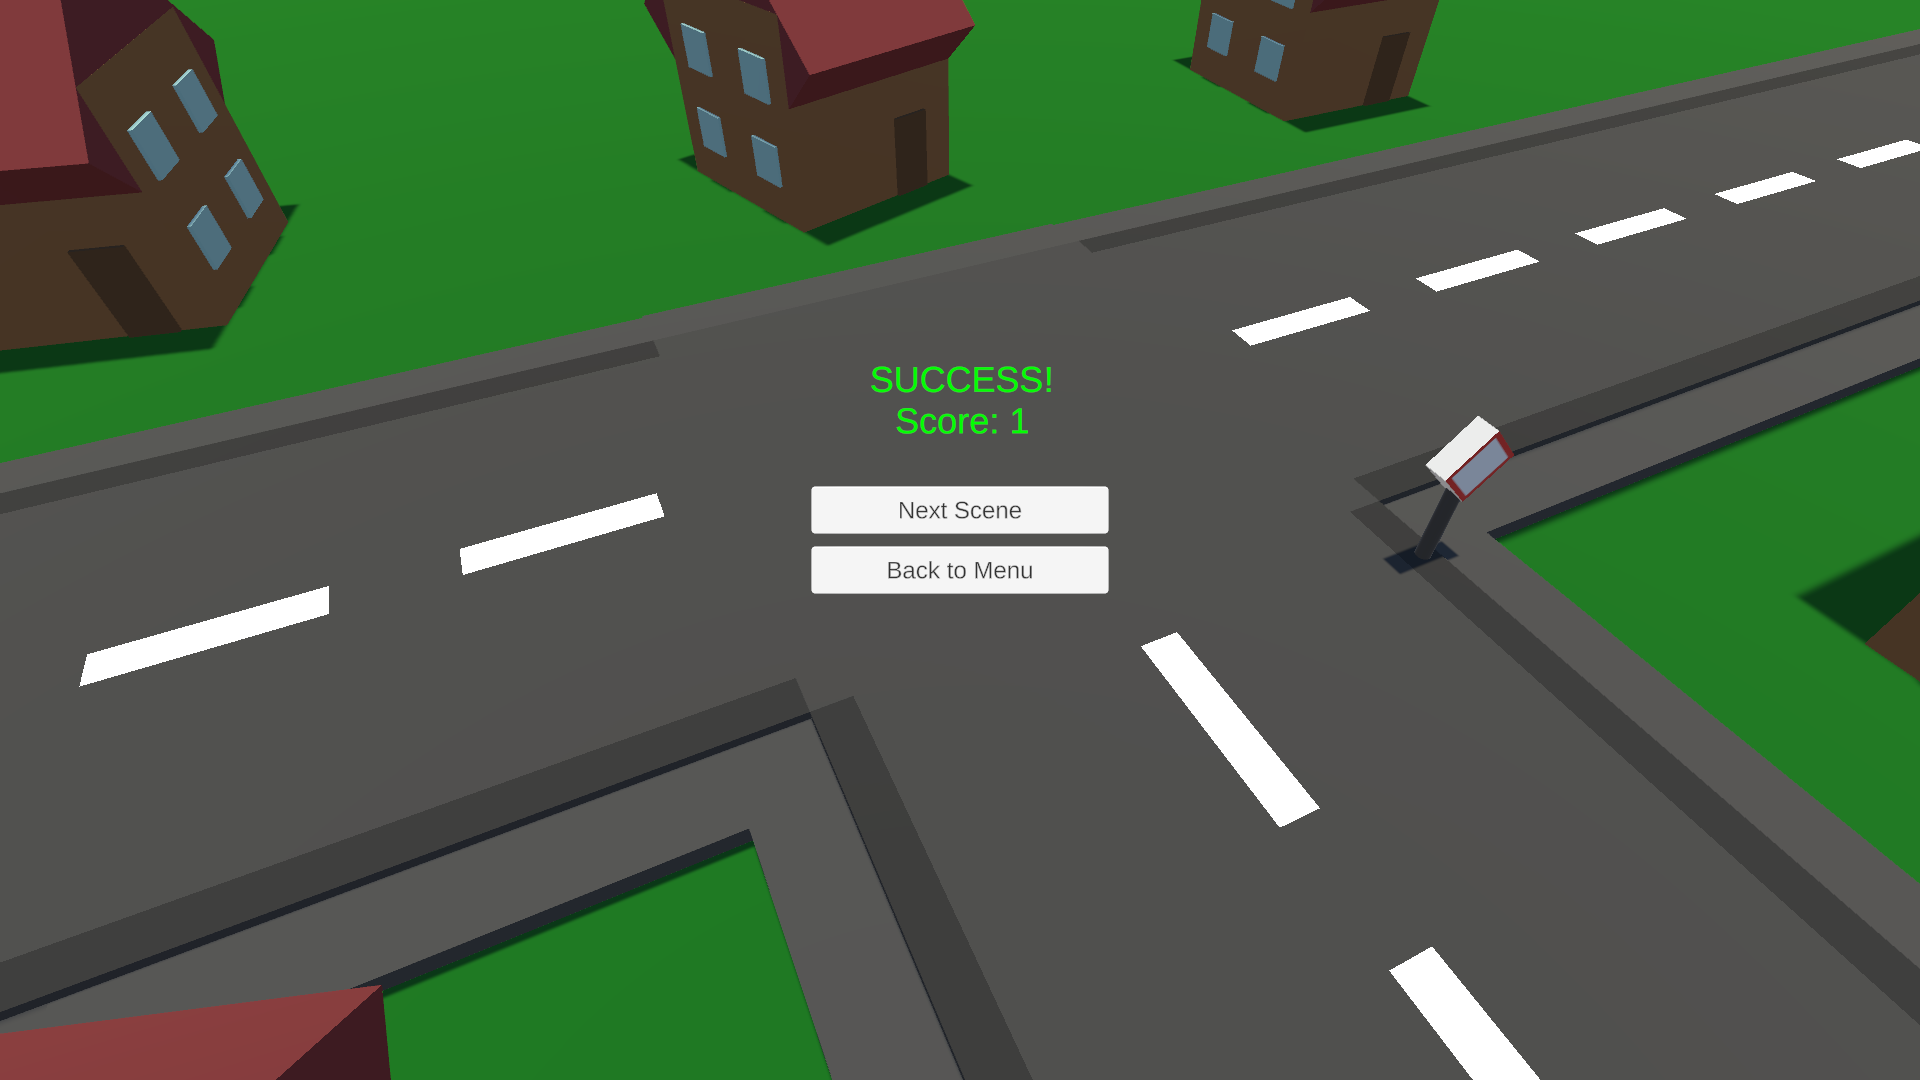
\includegraphics[height=5cm]{images/succes}
	\caption{Sikeresen megoldott feladat a szabad játékban}
\end{figure}
 
\section{Teszt játék}
A ,,Teszt'' gombra kattintva egy teszt játék veszi kezdetét. A \textit{KRESZ vizsga} mintájára, adott darab feladványt kell megoldania a játékosnak. Egy teszt feladatai már meghatározottabbak mint a szabad játék szituációi. Van több nehézségi szint. A különböző nehézségű feladatokat arányosan osztja el a rendszer, így a könnyebb és nehezebb szituációkkal egyaránt meg kell tudni birkózni a teszt teljesítéséhez.
\begin{itemize}
	\item Könnyű:
	\begin{figure}[ht!]
		\centering
		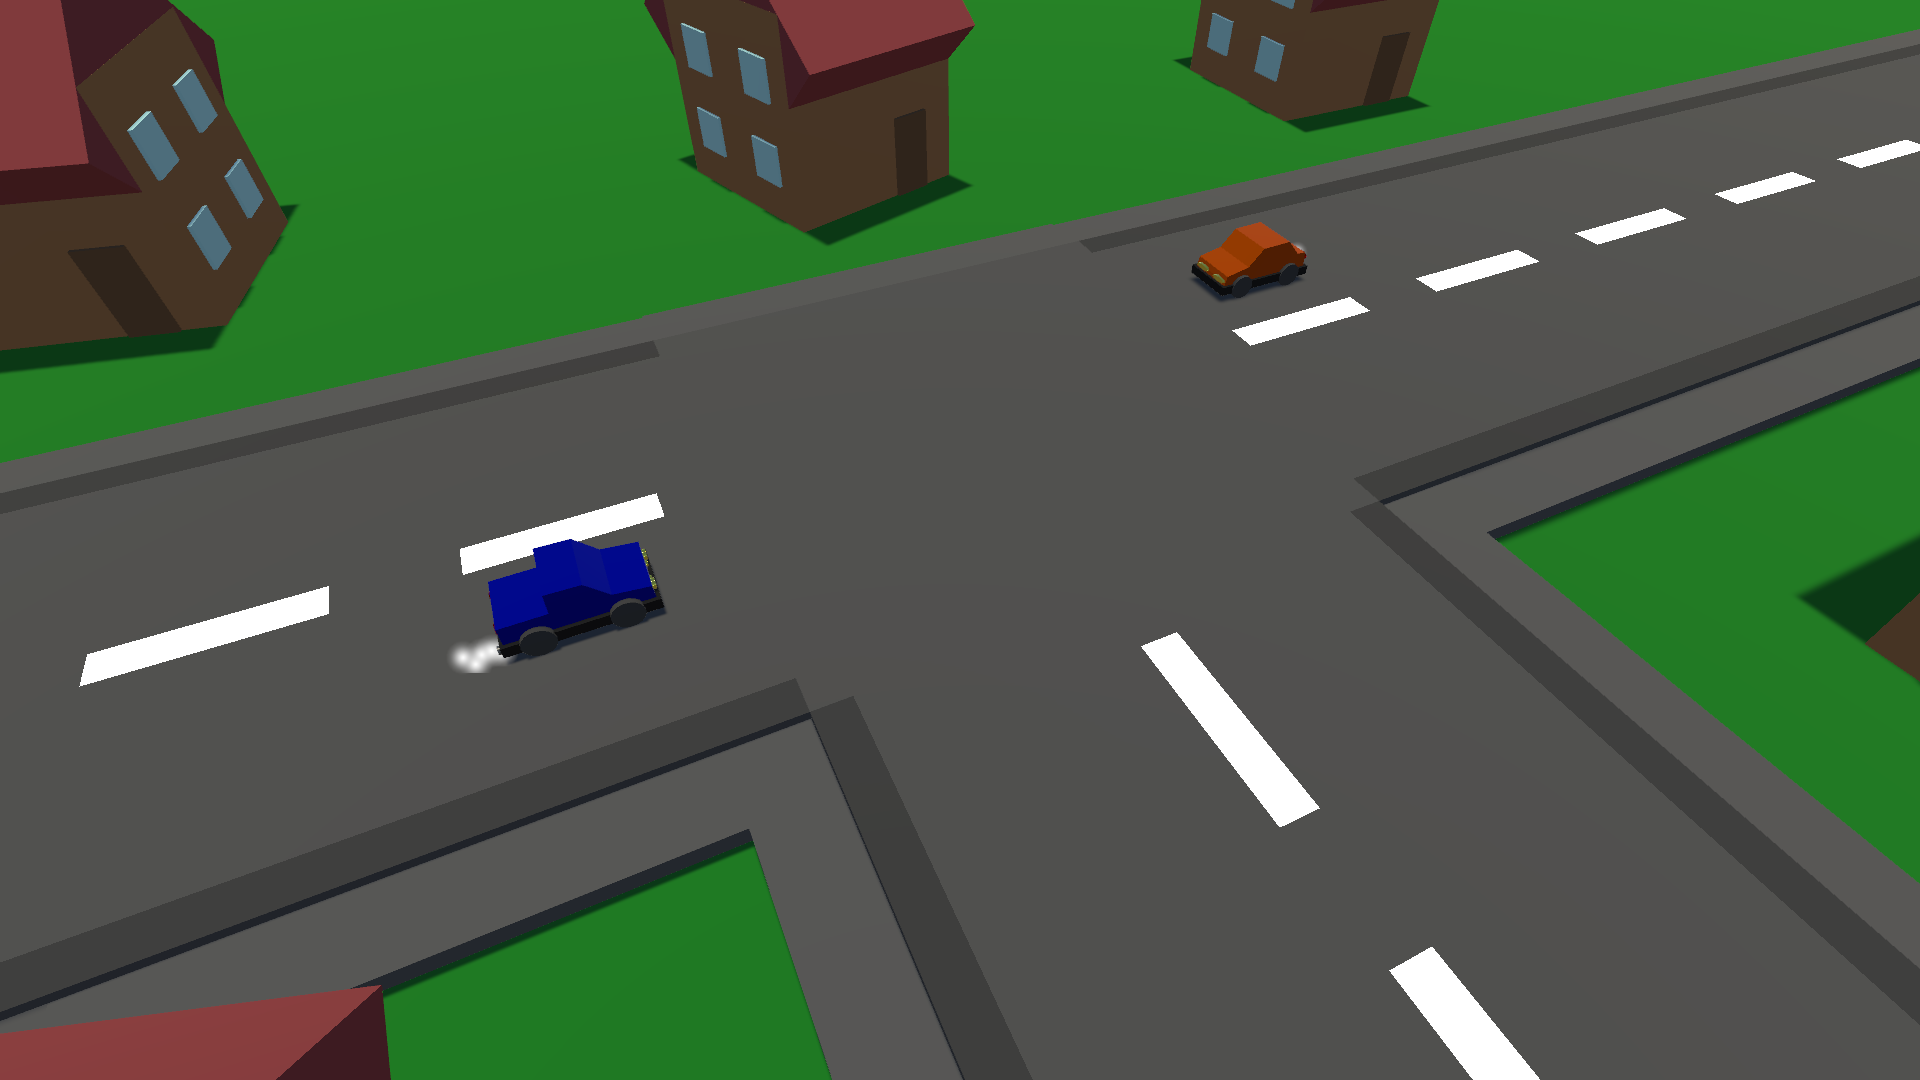
\includegraphics[height=5cm]{images/easy}
		\caption{Könnyű szintű feladat}
	\end{figure}
	\item Közepes:
	\begin{figure}[ht!]
		\centering
		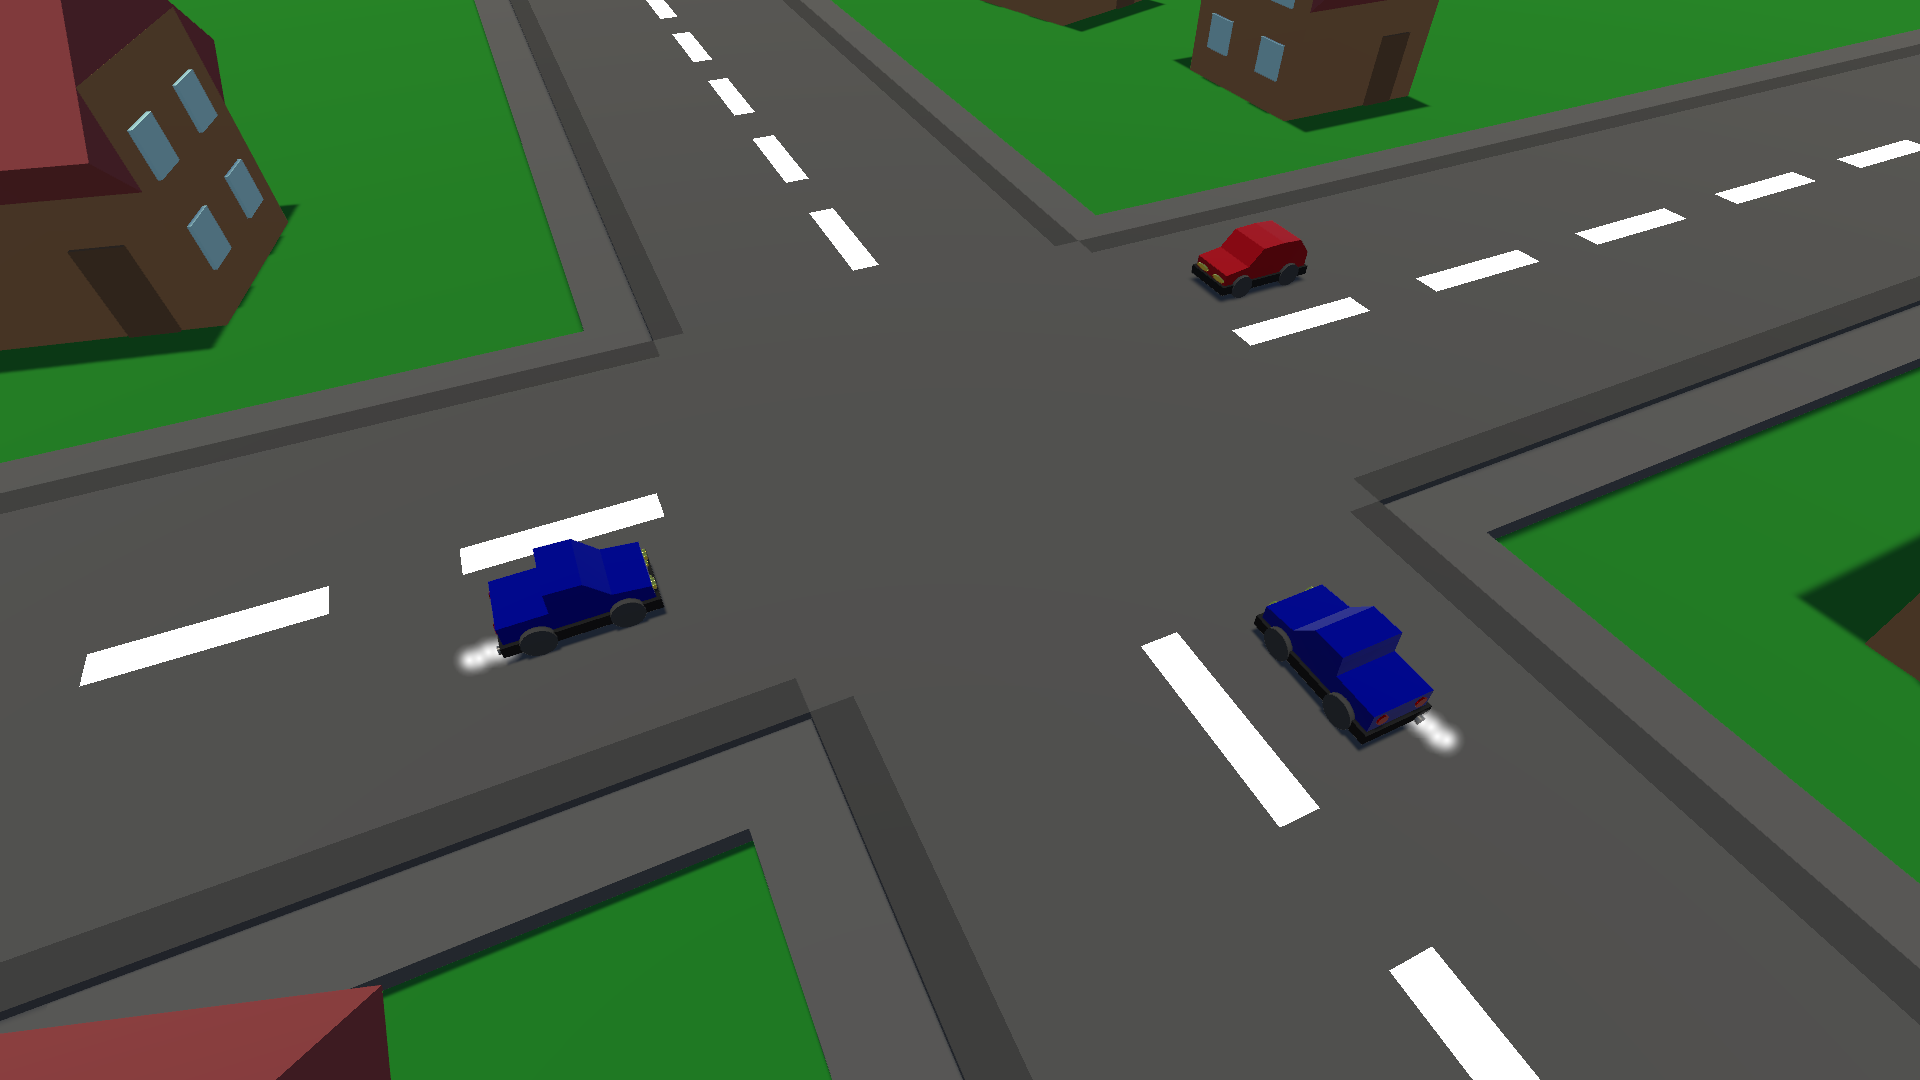
\includegraphics[height=5cm]{images/medium}
		\caption{Közepes szintű feladat}
	\end{figure}
	\item Nehéz:
	\begin{figure}[ht!]
		\centering
		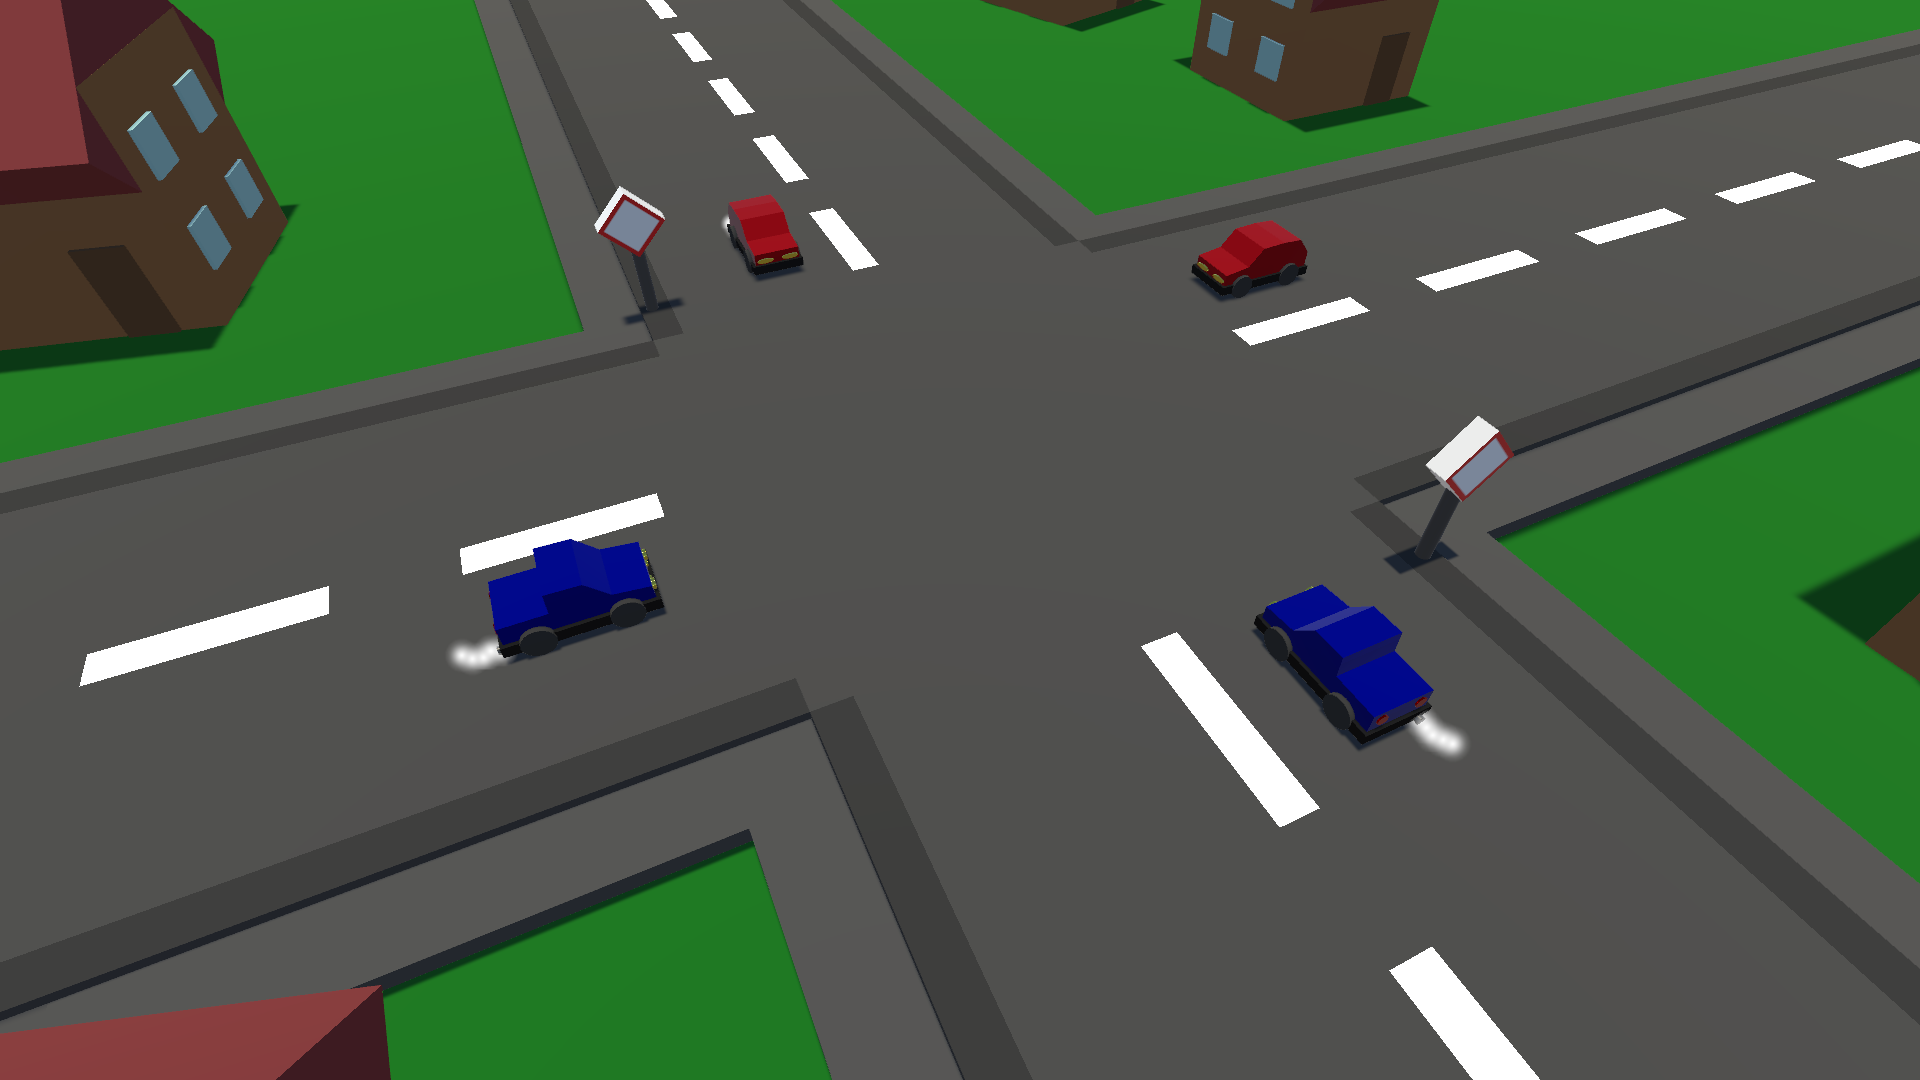
\includegraphics[height=5cm]{images/hard}
		\caption{Nehéz szintű feladat}
	\end{figure}
\end{itemize}
Itt is van pontrendszer, de itt már nem csak a rekordok fenntartása végett. A teszt sikeres teljesítéséhez, az összesen megszerezhető maximális pontszám legalább 90\%-át kell elérnie a játékosnak, de persze mindig lehet törekedni a tökéletes eredményre.

\begin{figure}[ht!]
	\centering
	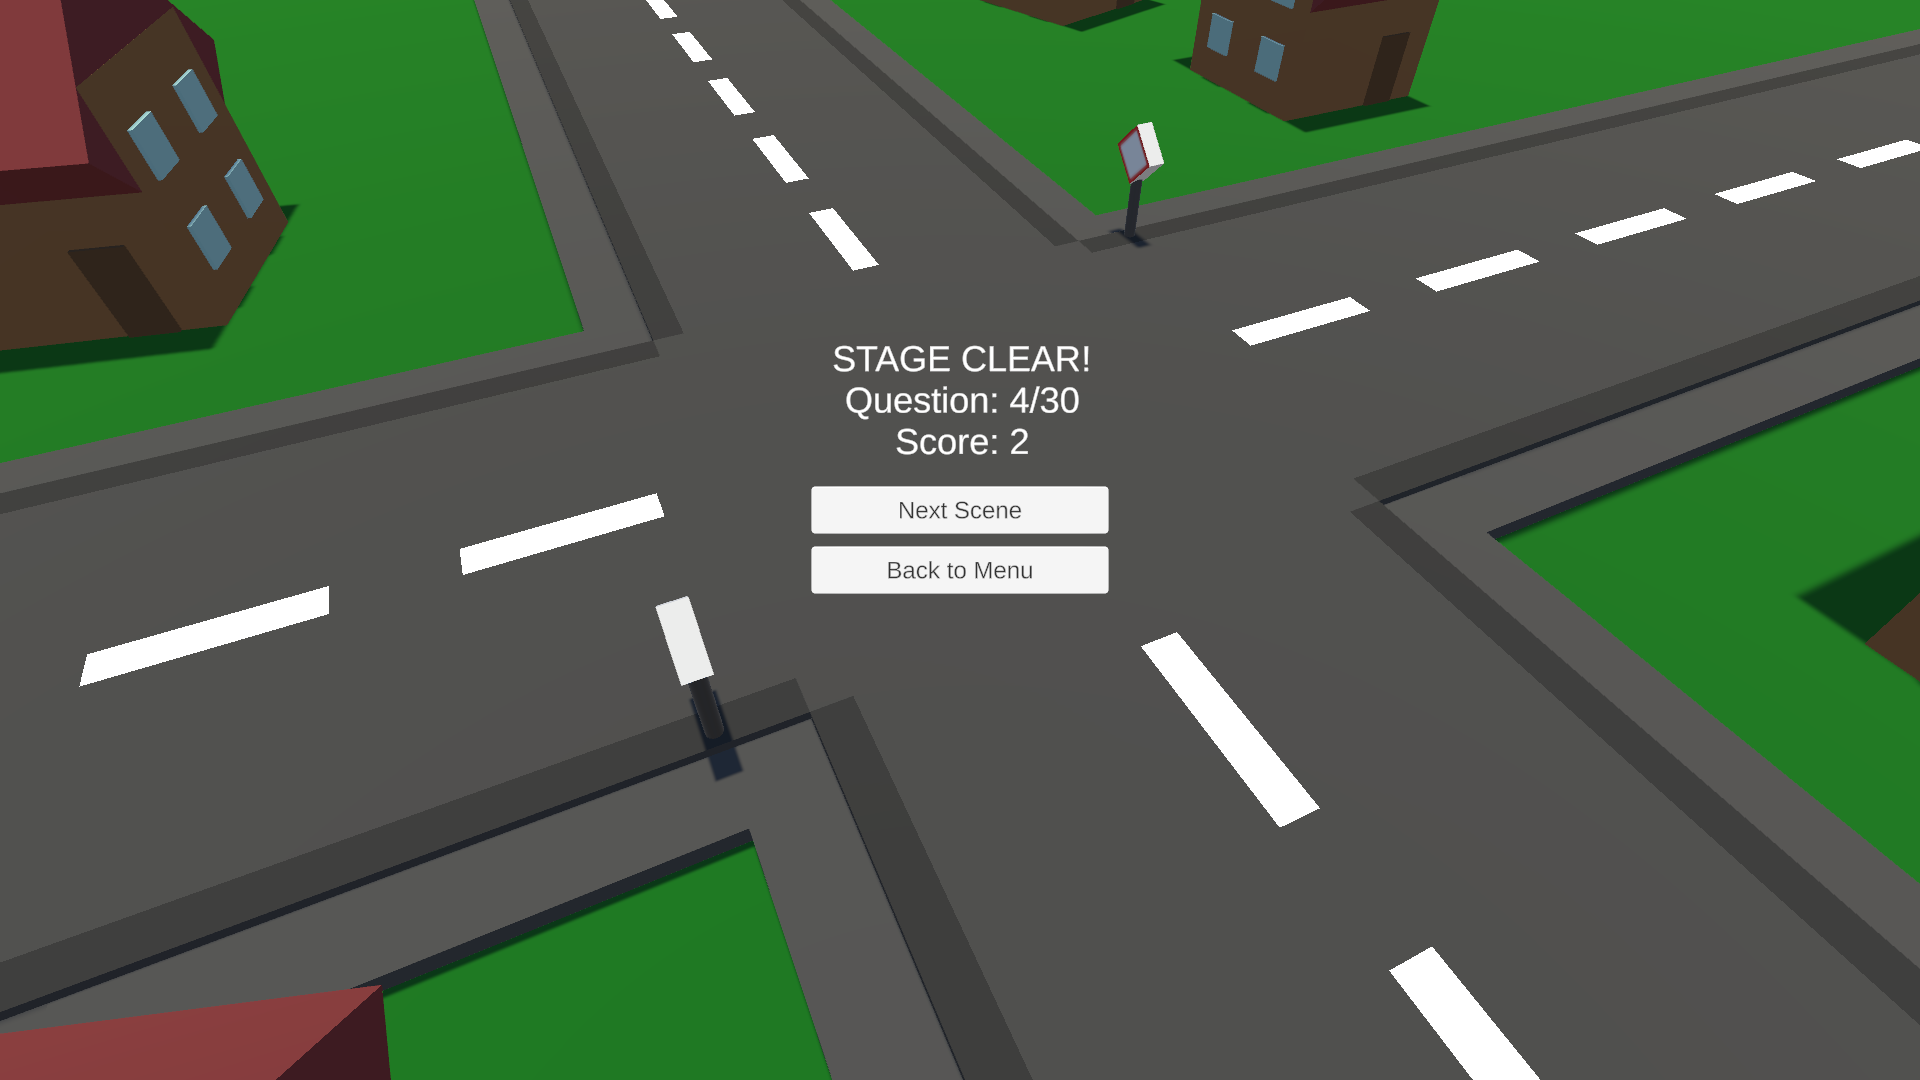
\includegraphics[height=5cm]{images/test}
	\caption{A Teszt játék köztes menüje egy sikeres feladatmegoldás után}
\end{figure}


\chapter{Saját szoftver}

\section{Fejlesztési idővonal}
A programom teljes kifejlesztése összesen 2 évet vett igénybe. Ez idő alatt voltak aktívabb és passzívabb időszakok is, volt amikor egy-egy áttörés után rövid időre megnövekedett az elért mérföldkövek száma. A program több alakot is öltött. 
\subsection{Tanulási időszak}
Az első félév alatt a program elég csekély formában volt jelen. Ebben az időszakban a fókusz a projekthez használt programozási nyelv megértésén és elsajátításán volt. 

Elkészültek a program első tervei amik később támpontot adtak a fejlesztés során. Már itt előre sok elméleti problémára próbáltam megoldást keresni, ötletelni, hogy ha esetleg ezek a problémák később felmerülnének, ne érjen akkora meglepetés.
\subsection{Szoftver alapok}
A program első verziója még teljesen a \textit{Visual Studio}-ban, egy ,,WinForms'' felületre készült. Itt jött létre a program alapjául szolgáló algoritmus első, primitív verziója, ami a szituációk előre megadott adatokból volt képes kiszámolni az áthaladás megfelelő sorrendjét.

Ebben az állapotban még csak az alapszabályoknak megfelelően működött, nem tudta még kezelni a nem teljesen lineáris megoldásokat. A kiválasztott paraméterek alapján felállított egy sorrendet és azt adta vissza a kezelőfelületen, nem volt még vizuális megjelenítés, csak számok és szavak.
\subsection{Unity alapok}
A második félév végén nagy áttörés történt. A program átköltözött a Unity keretrendszerébe. Az eddig kifejlesztett algoritmus megkapta az interaktív felületet az első vizuális megjelenítését. Ez már a GitHubra is felkerült.

A harmadik félévben rájöttem, hogy habár a programíráshoz már megvan a tudásom, a Unity sajátos eszközkészletét még messze nem ismerem eléggé. Tanuló anyagokat kerestem a témában, gyakorló projekteket hoztam létre, és teljesítettem egy Unity specifikus kurzust is, hogy a megfelelő szintre hozzam a tudásomat, mindemellett folyamatosan integráltam az ezalatt tanult módszereket és újdonságokat a programba. 
\subsection{Legfrissebb verzió}
Az utolsó pár hónapban is sok módosításon esett átt a játék. Elkészült egy kezdetleges ,,feedback'' rendszer ami a későbbiekben lényegesen megkönnyítette a hibakeresést és a javítást, hiszen a konzolon folyamatosan megjelentek a ,,real time'' adatai az aktív feladatnak. Később pedig az eredetileg \textit{placeholder}-nek szánt modellek is lecserélésre kerültek.

Az algoritmus finomodott és immár képessé vált a nem lineáris sorrendű megoldások kezelésére. Ez gyakorlatban annyit jelent, hogy az algoritmus folyamatosan újravizsgálja a szituációt minden lépés után, és megállapítja a következő helyes válaszlehetőségeket. Erről még bővebben később.
\section{Menü}
A játékban kétféle menü van. A Főmenü és a köztes játékmenü.
\begin{itemize}
	\item Főmenü, egyszerű 3 gombbal rendelkezik:
	\begin{itemize}
		\item Play: Elintítja a szabad játék módot.
		\item Test: Elindítja a teszt játék módot.
		\item Exit: Kilép a játékból, bezárja azt.
	\end{itemize}
	\item Játékmenü
	\begin{itemize}
		\item Next Scene: Továbblép a következő feladatra.
		\item Back to Menu: Kilép a főmenübe. Ez mindkét játékmód esetében az alaphelyzetbe helyezi az előrehaladást.
	\end{itemize}
\end{itemize}
\section{Játékprogram}
A projekt fő része, játék alapjaként szolgáló program, 3 fő részből áll:
\begin{itemize}
	\item Utak
	\item Járművek
	\item Kereszteződések
\end{itemize}
Az utak és a járművek alkotják a kereszteződéseket, utóbbiak pedig az előbbiek adataiból elvégzik a szituációk létrehozásához kellő számításokat, és kezelik a megoldó algoritmust.
\subsection{Utak}
Elindítjuk a játékot, a jelenet futni kezd, a \textit{Road} osztály az első megálló. 

\begin{itemize}
	\item Létrehozza a \textit{Node}-okat.
	\begin{itemize}
		\item \textit{StartNode}: Az út objektumok jobb oldalán található Node. Ez a jámrművek kiindulási pontja, itt jelennek meg először.
		\item \textit{EndNode}: Az út bal oldalán található Node. Ide érkeznek a járművek, ez a kilépési pontjuk. Ez a Node határozza meg az adott jármű irányát.
	\end{itemize}
	\item Megjelöli a felhasznált út objektumok irányát. Innen érkezik az az információ, hogy a jármű melyik utak Start- és EndNodejai közül választhat.
	\item Kiosztásra kerülnek az út rangok. Később ez alapján érvényesülnek az elsőbbség, és jobbkéz szabályok. Ha egy út magasabb rangú mint a szomszédja akkor az azon úton haladó jármű elsőbbséget élvez az alacsonyabb rangú úton állóval szemben. Ha az utak egyenrangúak, a jobbkéz szabály érvényesül.
	\item A \textit{PlaceVehicle} metódus a \textit{Vehicle} osztályból beérkező adatokkal egy járművet hoz létre, amit elhelyez az út \textit{StartNode}-ján.
\end{itemize}
\begin{figure}[ht!]
	\centering
	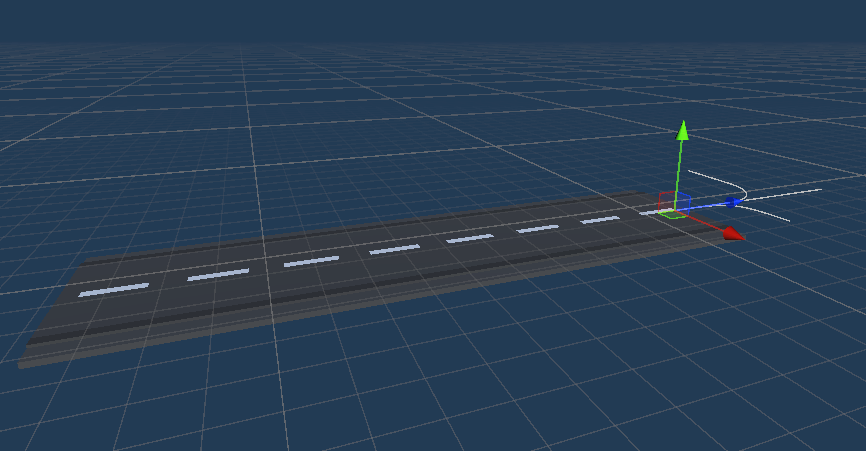
\includegraphics[height=5cm]{images/road}
	\caption{Egy út objektum felépítése}
\end{figure}
\subsection{Járművek}
A második megálló a \textit{Vehicle} osztály.
\begin{itemize}
	\item Létrejön egy jármű objektum, és a következő paramétereket kapja meg:
	\begin{itemize}
		\item \textit{Kiindulópont}: Egy olyan \textit{StartNode} ami szabad.
		\item \textit{Irány}: Lehet előre, balra vagy jobbra.
		\item \textit{Cél}: Az alapján, hogy melyik irányba szeretne haladni, megkapja az annak megfelelő \textit{EndNode} adatait. EndNode lehet közös, StartNode nem.
		\item Jobb szomszéd: Megvizsgálja van e tőle jobbra másik jármű, hiszen egyenrangú kereszteződés esetén el kell engednie.
		\item Rang: Ez a járművek rangja, a játék közben folyton változik ahogy a járművek megközelítik, majd elhagyják a kereszteződést. Ez adja meg az áthaladási sorrendet. Azért kell folyamatosan frissülnie, mert némelyik szituációban lehet több aktuálisan helyes lépés is, valamit egy lépés után lehet olyan jármű aki elveszíti a szomszédját. 
		\item Az animációkhoz használt komponensek is itt csatolódnak az objektumokhoz. \cite{unity_monobehaviour}
	\end{itemize}
	\begin{figure}[ht!]
		\centering
		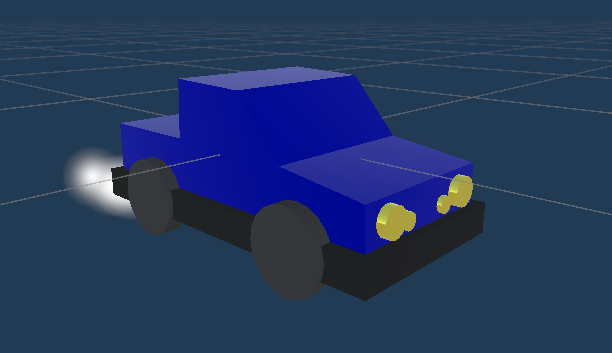
\includegraphics[height=5cm]{images/jarmu}
		\caption{A járművek egyik modellje}
	\end{figure}
\end{itemize}
\newpage
\subsection{Kereszteződések}
A kereszteződéseknek két része van. Az \textit{IntersectionBuilder} osztály és az \textit{IntersectionSolver} osztály.
\begin{itemize}
	\item \textit{IntersectionBuilder}: ,,Megépíti'' a kereszteződéseket. Felhasználva a kész út és jármű objektumokat és azok paramétereit, az elemeket összerakva vizualizálja a kész \textit{Itersection} objektumot. Egy ilyen objektumnak legalább két járműből és három útszakaszból kell állnia, hogy megfelelő kereszteződést alkosson.
	\item \textit{IntersectionSolver}: 
	\begin{itemize}
		\item Kezeli a megoldó algoritmust, a folyamatosan frissülő áthaladási sorrendet és az alapján Log-ol a konzolra is.
		\item Kezeli a rövid és hosszútávú eredményeket a pontszámrendszerrel a szabad játék és a teszt játék esetében is.
	\end{itemize}
	\begin{figure}[ht!]
		\centering
		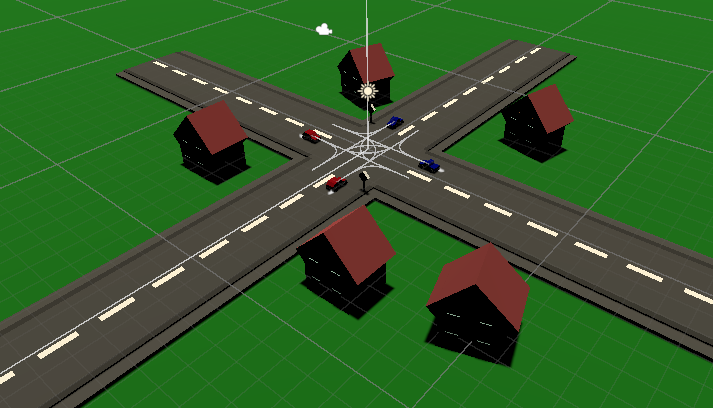
\includegraphics[height=5cm]{images/keresztezodes}
		\caption{Egy éppen aktív kereszteződés}
	\end{figure}
\end{itemize}
\chapter{Fejlesztési lehetőségek}
Rengeteg potenciál van még a programban. Sok olyan ötletem volt és van ami még nem valósult meg, de elméletben már létezik.
\section{Textúrák és modellek}
A projekt alatt sokkal több figyelmet fordítottam a program működési folyamatainak megbízhatóságára mint a megjelenésére, így van még pár olyan része a játéknak amire ráférne egy ráncfelvarrás:
\begin{itemize}
	\item Autók: A játék kis szereplői, a közlekedésben részvevő járművek habár aranyosak a maguk alacsony bonyolultságú kinézetükkel, sokat hozzátenne a játékélményhez az alaposabban kidolgozott autó modellek alkalmazása. A fejlesztendő textúrák és modellek közül ez számomra a legfontosabb, és ez egy hozzáértő új csapattag bevonásával könnyen megvalósítható lenne.
	\begin{figure}[ht!]
		\centering
		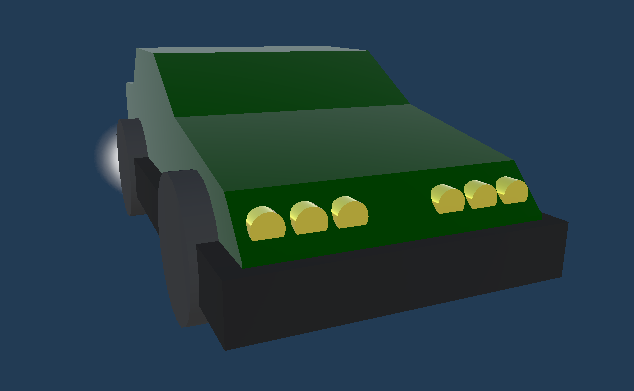
\includegraphics[height=5cm]{images/jarmu2}
		\caption{A járművek egyik modellje, amit lehetne fejleszteni}
	\end{figure}
	\newpage
	\item Gombok és feliratok: A játék legtöbb felirata és gombjai egyszerű kinézettel rendelkeznek. Ezeknek a cseréje szintén nagyon feldobná a játékot és jobb esztétikai élményt adna.
	\item Környezet: A játékkörnyezet legalább annyira fontos mint a résztvevő autóké. A környezet kidolgozottsága egyeznie kell a járművekével, hogy az autók ne tűnjenek ki a helyzetből jobban mint kellene.
\end{itemize}

\section{Új pályák és szituációk}
Szeretném, hogy a játék ne legyen túlságosan egyoldalú. Ennek az eléréséhez a jövőben új pályákat tervezek hozzáadni amik egy fokkal feljebb emelik az alap kereszteződés alapú pályákat.

A kereszteződések mellett a következő lépés a kétirányú úttestek, körforgalmak és lámpás kereszteződések, esetleg további résztvevő járművek integrálása lesz.

\begin{figure}[ht!]
	\centering
	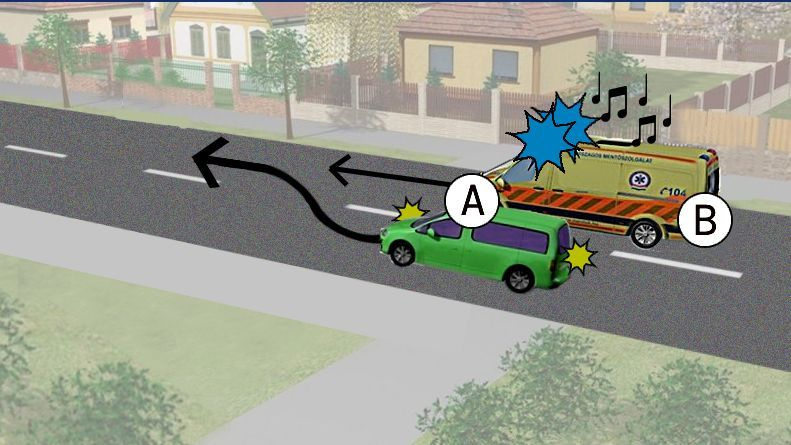
\includegraphics[height=5cm]{images/mento2}
	\caption{KRESZ feladat mentőautóval \cite{mento2}}
\end{figure}

A nehézségi szintet tovább emelve, a járműveknek \textit{Collidert} adva az áthaladási animációkkal egyszerű baleseteket is szimulálhatnánk, ami türelemre és odafigyelésre is tanítaná a játékost.
\section{Új szabályrendszerek}
Az új kétirányú, körforgalom és lámpás kereszteződések beépítésével új szabályrendszerekre is szükség lesz.
\begin{itemize}
	\item Kétirányú úttest: Az ilyen típusú pályához kell egy olyan algoritmus ami tudja szimulálni az előzés, kikerülés, úttest elhagyása és a megkülönböztető jelzéssel haladó jármű érkezését, és az ezek által létrehozott szimulációban a kereszteződésekhez hasonlóan áthaladási sorrendet és megoldást generálni.
	\item Körforgalom: A Körforgalom egy egyszerű de annál furfangosabb és fontos része a közúti közlekedésnek. A beépítéséhez egy külön elsőbbség adási rendszer, és az irányjelzés és az azt figyelő algoritmus is része kell, hogy legyen.
	\begin{figure}[ht!]
		\centering
		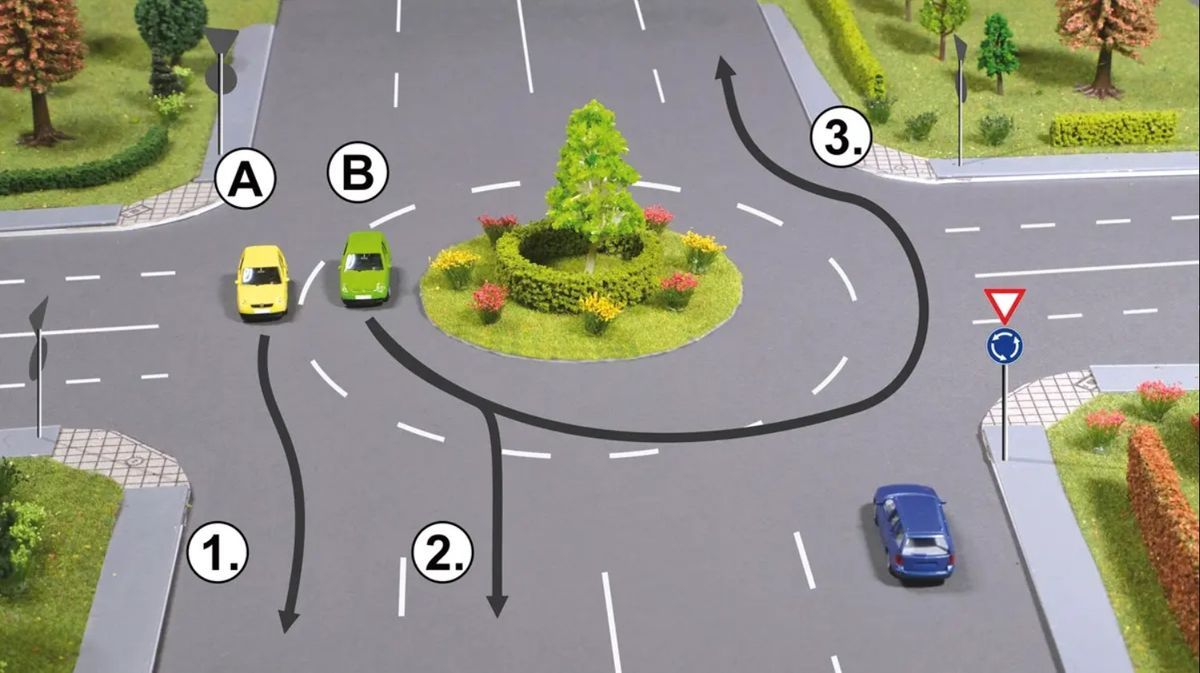
\includegraphics[height=5cm]{images/korforgalom}
		\caption{KRESZ feladat körforgalommal \cite{korforgalom}}
	\end{figure}
	\item Lámpás kereszteződés: A lámpás kereszteződés a mostanihoz hasonló de egy lépcsőfokkal ellenőrzöttebb rendszer, viszont fontosnak érzem, hogy a későbbiekben ez is a része legyen a programnak.
	\item Új járművek: A KRESZ-ben gyakran előfordulnak speciális járművek és résztvevők amikre a forgalom különös figyelemmel vagy akár konkrét szabályokkal reagál. Ilyen például:
	\begin{itemize}
		\item Vonat: Vasúti átkelőhely.
		\item Villamos: Kereszteződés villamossínnel, opcionális érkező villamossal.
		\item Megkülönböztető jelzés: Rendőr, mentő, tűzoltó! A kereszteződésekbe és többi pályaformába is opció.
		\item Gyalogos: Sok esetben nem teljesen egyértelmű, hogy egy gyalogosnak mikor van elsőbbsége az autókkal szemben, és ez könnyen bezavarhat egy-egy szituációban, így extra nehezítésként a gyalogosok jelenlétét is lehetne adni a feladathoz.
	\end{itemize}
	\begin{figure}[ht!]
		\centering
		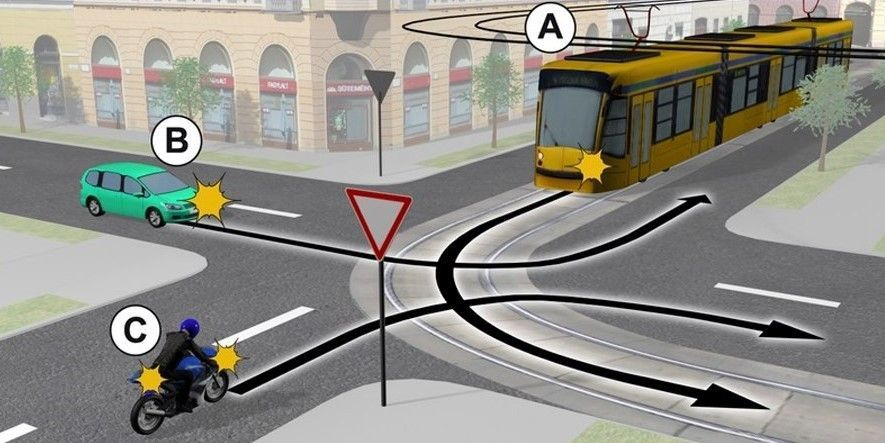
\includegraphics[height=5cm]{images/villamos}
		\caption{KRESZ feladat villamossal \cite{villamos}}
	\end{figure}
	\begin{figure}[ht!]
		\centering
		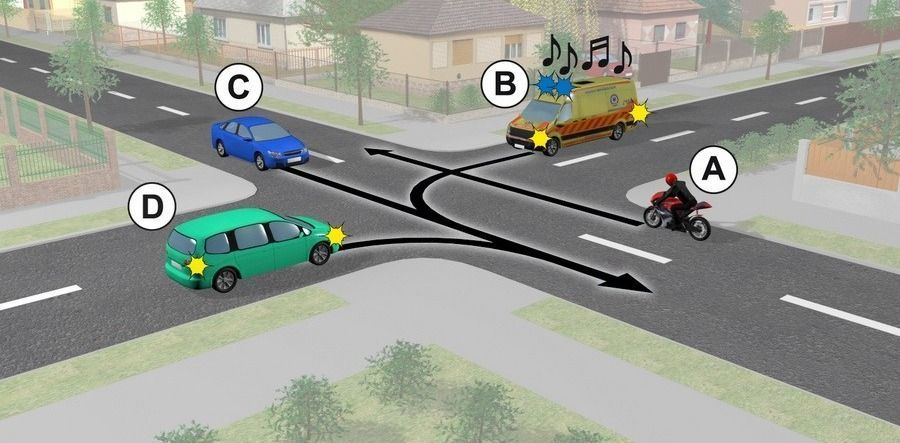
\includegraphics[height=5cm]{images/mento}
		\caption{KRESZ feladat mentőautóval \cite{mento}}
	\end{figure}
\end{itemize}
\newpage
\section{Szabálylista}
A játékon belül egy olyan felület, ahol a játék során fellelhető közlekedési szabályokat magyarázattal és illusztrációval vannak feltüntetve. Így ezeket a szabályokat a programon belül tanulmányozhatja a felhasználó, ha valamelyiknek szeretne utánanézni esetleg egy elrontott feladat után.
\section{Testreszabható feladatok}
Még az első bővítési ötleteim között volt a szituációk testreszabhatósága. Ez azt jelentené, hogy egy külön játékmódban a felhasználó beállíthatja, hogy:
\begin{itemize}
	\item Milyen kereszteződés vagy közlekedési helyzet legyen a szituáció alapja.
	\item Milyen és hány résztvevője legyen az adott feladatnak.
	\item Az adott résztvevők milyen irányban haladjanak tovább, rendelkezzenek e bármilyen plusz joggal.
\end{itemize}
A beállítások véglegesítése után a játékos megoldhatja a saját szituációját aztán pedig új feladat létrehozásába kezdhet.
\chapter{Tesztelés}
A programozás egyik elengedhetetlen része a tesztelés. A projektem fejlesztése során kétféle tesztelési módszert alkalmaztam: Manuális és egységtesztek, másik nevén \textit{Unit tesztek}. 
\section{Manuális}
A manuális tesztelés során olyan funkciókat vizsgálok, mint például a bemenet, megjelenítés, vagy a menü különböző gombjainak működése. A fejlesztés közben folyamatosan csináltam manuális teszteket. Minden új funkciót rögtön tesztelni kell, hogy megfelelően működik, így nagyon gyorsan kiszűrhetőek az esetleges hibák.

Később már végeztem nagyobb, teljes rendszer szintű manuális teszteket is, ahol egyben az egész játékot teszteltem, és nem csak a legfrissebb funkciókat. Ez azért fontos mert egy hosszabb fejlesztés után ha egy-egy funkció jól is működik, nem akadályozhatják egymást.
\begin{figure}[ht!]
	\centering
	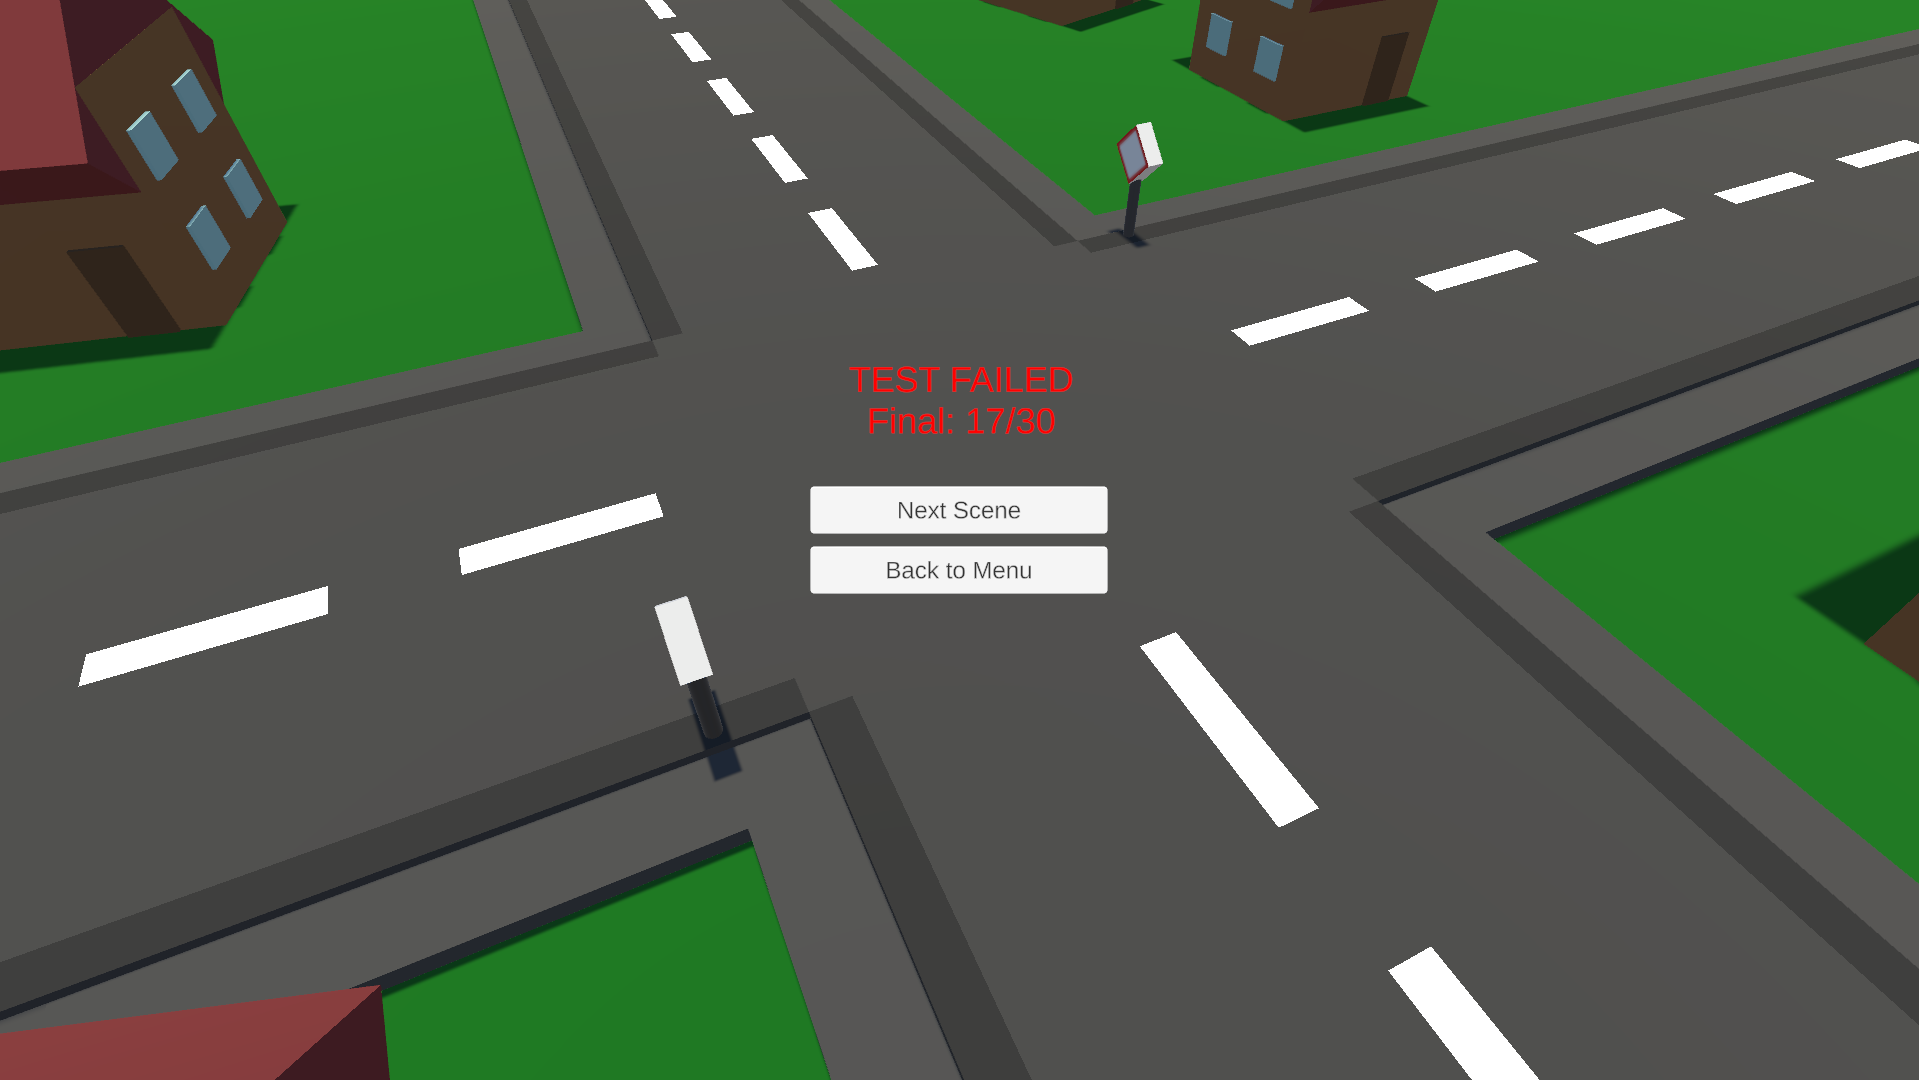
\includegraphics[height=5cm]{images/test_fail}
	\caption{Manuális tesztelés (Teszt játék, nem elég pont)}
\end{figure}
\newpage
A manuális tesztek eredményei:
\begin{itemize}
	\item A szabad játék és a teszt játék pontrendszere is megfelelően működik és minden esetben helyesen írja ki az aktuális értéket.
	\item Az animációk megfelelően és simán futnak végig.
	\item A megoldó és sorrend felállító algoritmusok megfelelően működnek. Felismerik az esetleges egyenrangúságot a járművek esetében és tudják kezelni.
	\item A Főmenü és a játékmenü gombjai is megfelelően működnek.
\end{itemize}
\section{Egységteszt}
Az egységtesztek olyan tesztek amiket a programunk adatokkal és változókkal foglalkozó részére írunk. Ezek a tesztek automatizáltak és azt tudjuk velük ellenőrizni, hogy a szoftver teljesíti e a feladatait.

A Unity keretrendszerben ezt egy külön package telepítésével tehetjük meg, a \textit{Test Framework}-el. A kezeléséhez megnyitjuk a tesztelő felületet, azaz a \textit{Test Runnert}. Két opciónk van:
\begin{itemize}
	\item Play Mode: Itt olyan teszteket tudunk csinálni amelyek futási időben dolgoznak. Ilyenkor a keretrendszer elindítja a játékot és úgy futtatja a teszteket.
	\item Edit Mode: Ebben a módban azok a kódrészek tesztelhetőek amelyek nem foglalkoznak a futásidő alatt aktív objektumokkal.
\end{itemize}
\chapter*{Összegzés}
\addcontentsline{toc}{chapter}{Összegzés}
A szakdolgozat végére úgy érzem, hogy az elképzelésem megvalósulni látszanak a kész programban. Eleinte úgy gondoltam, hogy sokkal egyszerűbb lesz, viszont ahogy haladtam előre a fejlesztésben, az újabb és újabb akadályok megmutatták mennyi belefektetett energiát is igényel egy ilyen program elkészítése. Rengeteg ötletem lenne még a program fejlesztésére, hogy milyen plusz funkciókat és elemeket tudnék beleépíteni a játékba. Ennek ellenére elégedett vagyok a program mostani állapotával is, hiszen mindig jó ha van hova fejlődni.

Tanulás szempontjából nagyon hasznosnak éreztem ezt a projektet. Rengeteg önfejlesztésen kellett átesnem, hogy elsajátítsam azt a tudást ami egy ilyen program fejlesztéséhez elengedhetetlen. Az 5.~fejezetben leírtakból szeretnék a lehető legtöbbet valamilyen módon a közeljövőben beépíteni a programba, ezáltal tovább fejlesztve és gyakorlással elmélyítve a tudásomat. 

Véleményem szerint ebből a programból nagyon hasznos eszköz válhat azok számára akik vezetni szeretnének tanulni és kell egy kis segítség a szabályok megértésében. A közlekedési szabályok megértése és gyakorlatban való alkalmazása rengeteg figyelmet és gyakorlást igényel, és nagyon fontos, hogy mindenki aki résztvesz a közlekedésben megfelelően fel legyen készítve a szabályok használatára.
\begin{thebibliography}{8}
\addcontentsline{toc}{chapter}{\bibname}
\bibitem{id_software}
\textsc{Wikipédia}: \emph{Id Software}, \url{https://en.wikipedia.org/wiki/Id_Software}, Megtekintve: 2026.04.05.
\bibitem{unreal_engine}
\textsc{Wikipédia}: \emph{Unreal Engine}, \url{https://en.wikipedia.org/wiki/Unreal_Engine}, Megtekintve: 2026.04.05.
\bibitem{godot_engine}
\textsc{Wikipédia}: \emph{Godot (game engine)}, \url{https://en.wikipedia.org/wiki/Godot_(game_engine)}, Megtekintve: 2026.04.05.
\bibitem{unity_engine}
\textsc{Wikipédia}: \emph{Unity (game engine)}, \url{https://en.wikipedia.org/wiki/Unity_(game_engine)}, Megtekintve: 2026.04.05.
\bibitem{unity_technologies}
\textsc{Wikipédia}: \emph{Unity Technologies}: \url{https://en.wikipedia.org/wiki/Unity_Technologies}, Megtekintve: 2026.04.06.
\bibitem{unity_components}
\textsc{Unity Documentation}: \emph{Introduction to components}: \url{https://docs.unity3d.com/Manual/Components.html}, Megtekintve: 2026.04.08.
\bibitem{unity_monobehaviour}
\textsc{Unity Documentation}: \emph{MonoBehaviour}: \url{https://docs.unity3d.com/ScriptReference/MonoBehaviour.html}, Megtekintve: 2026.04.08.
\bibitem{kresz}
\textsc{Wikipédia}: \emph{KRESZ}: \url{https://hu.wikipedia.org/wiki/KRESZ}, Megtekintve: 2026.04.18.
\chapter*{Ábrajegyzék}
\addcontentsline{toc}{chapter}{Ábrajegyzék}
\bibitem{harompontos}
\textsc{KRESZ vizsga}: \emph{Három pontos feladat}, \url{https://szuperjogsi.hu/images/slide/3/Bogi110.jpg}, Letöltve: 2026.04.20.
\bibitem{kresz_img}
\textsc{KRESZ Táblák}: \emph{Közlekedési táblák}, \url{https://vezess2.p3k.hu/app/uploads/2007/02/2123_19519_1000x700.jpg.jpg}, Letöltve: 2026.04.20.
\bibitem{villamos}
\textsc{KRESZ vizsga}: \emph{Három pontos feladat villamossal}, \url{https://www.beol.hu/helyi-eletstilus/2025/07/kresz-teszt-villamos-elsobbseg}, Letöltve: 2026.04.20.
\bibitem{mento}
\textsc{KRESZ vizsga}: \emph{Három pontos feladat mentőautóval}, \url{https://www.feol.hu/helyi-kozelet/2024/12/kresz-teszt-mentoauto}, Letöltve: 2026.04.20.
\bibitem{mento2}
\textsc{KRESZ vizsga}: \emph{KRESZ feladat mentőautóval}, \url{https://www.szon.hu/helyi-kozelet/2025/07/megelozheto-a-mento-a-legtobben-bebukjak-ezt-a-kerdest#google_vignette}, Letöltve: 2026.04.20.
\bibitem{korforgalom}
\textsc{KRESZ vizsga}: \emph{Három pontos feladat körforgalommal}, \url{https://www.beol.hu/helyi-eletstilus/2026/03/kresz-teszt-korforgalom}, Letöltve: 2026.04.20.
\bibitem{doom}
\textsc{DOOM}: \emph{DOOM képernyőkép}, \url{https://upload.wikimedia.org/wikipedia/en/thumb/d/de/Doom_ingame_1.png/250px-Doom_ingame_1.png}, Letöltve: 2026.04.20.
\bibitem{unreal_img}
\textsc{Unreal Engine}: \emph{Unreal Engine kezelőfelület}, \url{https://cdn2.unrealengine.com/ue5-modeling-mode-tech-blog-sandsculpting-2844x1559-1885809c9ebd.JPG}, Letöltve: 2026.04.20.
\bibitem{godot_img}
\textsc{Godot Engine}: \emph{Godot Engine kezelőfelület}, \url{https://upload.wikimedia.org/wikipedia/commons/e/e3/Godot3.4.png}, Letöltve: 2026.04.20.
\bibitem{unity_img}
\textsc{Unity Engine}: \emph{Unity kezelőfelület}, \url{https://unity.com/releases/2019-3/editor-tools}, Letöltve: 2026.04.20.
\end{thebibliography}

% Aláírt, szkennelt nyilatkozat beillesztése a szakdolgozat végére

\includepdf{nyilatkozat/nyilatkozat.pdf}
\end{document}